\documentclass[a4paper]{ctexart}

\usepackage{tabularx} % extra features for tabular environment
\usepackage{amsmath}  % improve math presentation
\usepackage{graphicx} % takes care of graphic including machinery
\usepackage[margin=1in,letterpaper]{geometry} % decreases margins
\usepackage{cite} % takes care of citations
\usepackage[final]{hyperref} % adds hyper links inside the generated pdf file
\usepackage{ctex}
\usepackage{titlesec}
%\usepackage{CJKutf8, CJK}
\usepackage{makecell}                 % 三线表-竖线
\usepackage{booktabs}                 % 三线表-短细横线
% \usepackage{natbib}
\usepackage{graphicx}				  % 表格单元格逆时针
\usepackage{multirow}				  % 合并单元格
\usepackage{array}
\usepackage{amssymb}				  % 勾
\usepackage{amsmath}
\usepackage{longtable}                % 导入 longtable 宏包,表格自动换行
\usepackage{caption}
\usepackage{subcaption}               % 设置子图
\usepackage{color}					  % 文本颜色包
\usepackage{xcolor}
\usepackage{bbm}					  % 输入指示函数
\usepackage{tablefootnote}			  % 表格注释
\usepackage{pythonhighlight}
%\usepackage{fancyhdr}
\usepackage{lastpage}
\usepackage{tocloft}
\usepackage{authblk}
\usepackage{setspace}

\usepackage[section]{placeins}

% 设置页面边距
\geometry{a4paper, top=1.7cm, bottom=1.6cm, left=1.6cm, right=1.6cm}

%\pagestyle{fancy}
%\fancyhf{}
%\fancyhead{}
%\fancyfoot{}
%\fancyhead[R]{\small Page \thepage\ of \pageref*{LastPage}}
%\fancyhead[L]{\zihao{-5} \songti 开题报告}

\usepackage{listings}                 % 导入代码块
\usepackage{xcolor}
\lstset{
	numbers=left, 
	tabsize=1,
	columns=flexible, 
	numberstyle=  \small, 
	keywordstyle= \color{ blue!70},
	commentstyle= \color{red!50!green!50!blue!50}, 
	frame=shadowbox, % 阴影效果
	rulesepcolor= \color{ red!20!green!20!blue!20} ,
	escapeinside=``, % 英文分号中可写入中文
	xleftmargin=2em,
	xrightmargin=2em, 
	aboveskip=1em,
} 

\hypersetup{
	colorlinks=true,       % false: boxed links; true: colored links
	linkcolor=blue,        % color of internal links
	citecolor=blue,        % color of links to bibliography
	filecolor=magenta,     % color of file links
	urlcolor=blue         
}
%++++++++++++++++++++++++++++++++++++++++
\titleformat{\section}{\Large\bfseries}{\thesection}{1em}{}
\titleformat{\subsection}{\large\bfseries}{\thesubsection}{1em}{}
\titleformat{\subsubsection}{\normalsize\bfseries}{\thesubsubsection}{1em}{}
\titleformat{\paragraph}[runin]{\normalsize\bfseries}{\paragraph}{1em}{}
\titleformat{\subparagraph}[runin]{\normalsize\bfseries}{\subparagraph}{1em}{}

\begin{document}
	
	
	\title{\songti \zihao{4}5月工作汇报}
	\author{\textrm{Ku Jui}}
	\date{\textrm{May 2024}}
	\maketitle
	
	\renewcommand{\figurename}{Figure} % 可以重新定义abstract,因为ctex会覆盖thebibliography
	% 	\begin{abstract}
		%		In this experiment we studied a very important physical effect by measuring the
		%		dependence of a quantity $V$ of the quantity $X$ for two different sample
		%		temperatures.  Our experimental measurements confirmed the quadratic dependence
		%		$V = kX^2$ predicted by Someone's first law. The value of the mystery parameter
		%		$k = 15.4\pm 0.5$~s was extracted from the fit. This value is
		%		not consistent with the theoretically predicted $k_{theory}=17.34$~s. We attribute %this
		%		discrepancy to low efficiency of our $V$-detector.
		%	\end{abstract}
	
	\renewcommand{\tablename}{Table}
	
	% 设置目录标题为居中
	\renewcommand{\cfttoctitlefont}{\hfill\Large\bfseries\songti}
	\renewcommand{\cftaftertoctitle}{\hfill}
	\renewcommand{\contentsname}{Content}
		
	\tableofcontents
	
	\newpage	
	
%	\section{摘要}
%	
%		低光图像增强(LLIE)旨在增强图像亮度并恢复低光图像细节。然而,现有基于深度学习的LLIE模型仍面临诸如信息丢失、细节恢复不足、噪声、色差和细节失真等挑战,导致无法准确恢复低光图像(LLI)中的暗部细节,且模型往往过于复杂且存在冗余。为了解决这些问题,本文提出了一种简单而有效的LLIE模型,称为上下文网络(xxx-Net)。该模型由两个核心部分组成:1) 基于U-Net架构的编码器和解码器,用于处理图像的整体结构;2) 位于模型中心的BottleNeck块,由Swin Transformer块组成,用于捕获弱光图像的全局上下文信息。此外,我们还引入了即插即用的Cbam块,以学习和强调弱光图像中的局部细节。通过大量实验,我们证明了xxx-Net在恢复低光图像的暗部区域方面具有出色的性能,同时具有较少的参数和更快的推理速度,从而在低光图像增强任务中取得了显著的进步。
%	
%	\section{引言}
%		
%		低光图像增强(Low-Light Image Enhancement, LLIE)是视觉监控、自动驾驶和计算摄影等领域的重要应用之一。低光条件下拍摄的照片常常会遭受多种退化现象,如低对比度、可见度不足、噪声和色彩失真,这些问题不仅影响视觉感知,还会干扰后续的高级图像处理任务。因此,低光图像增强是图像处理领域的一个关键任务,旨在提升低光环境下拍摄图像的视觉质量。近年来,该领域的发展主要受到深度学习技术的驱动,涉及多种学习策略、网络架构、损失函数和训练数据集的运用。然而,在低光图像中恢复照度并精确恢复极暗区域的细节信息依然是一项充满挑战的任务。
%		%尤其在智能手机摄影领域,由于相机光圈大小、实时处理需求和存储限制,低光环境下的图像拍摄面临着显著挑战。
%		为应对这一挑战,研究人员提出了众多LLIE方法,包括传统方法和基于深度学习的方法。
%		
%		
%		%介绍传统的低光图像增强方法
%		传统的低光图像增强技术,如基于直方图均衡化\cite{ji1994adaptive}和Retinex理论\cite{land1965, land1977retinex, jobson1997properties}的方法,能在一定程度上提升图像的视觉质量。这些方法通常依赖于各种图像先验来构建模型,以逆向恢复退化的图像。然而,尽管这些传统技术能够增强图像的整体对比度,它们往往也会加剧背景噪声的对比度,同时减弱有价值的图像细节的对比度,从而影响最终的视觉效果。%Retinex算法旨在消除图像照度分量的干扰并还原图像真实色彩,但通常忽略噪声问题,可能导致增强结果中噪声的保留或放大,并且其复杂的优化过程增加了模型的复杂度。	
%		%传统的低光增强方法,如基于直方图均衡\cite{ji1994adaptive}和 Retinex\cite{land1965, land1977retinex, jobson1997properties}的方法,直方图均衡化重新调整图像的直方图分布,一方面增加了图像的全局对比度,另一方面使得亮度在整个图像的分布更加均匀。直方图均衡化的方法非常快速有效,并且是一个可逆操作,但缺点在于其不加选择地处理数据,可能增加背景噪声的对比度,同时降低有用的图像内容的对比度,导致视觉效果欠佳。此外,该方法也无法适用于复杂多变的低光照场景。Retinex 算法的核心思想是消除源图像照度分量干扰,依据反射分量信息还原图像真实色彩。基于 Retinex 的方法能够很大程度改善图像质量,但在应用的过程中仍存在不可忽视的缺点。例如,其通常忽略噪声问题,可能导致增强结果中噪声的保留或放大;有效的先验或正则化的选择具有挑战性,不准确的先验可能导致伪影和颜色偏差;此外,这些方法的复杂优化过程也导致最终的模型较为复杂。
%		近年来,基于深度学习的低光图像增强技术取得了显著成就,其通过设计各种模块和损失函数来学习从低光图像到正常光图像的映射。由于深度学习方法强大的学习能力,往往能够产生更好的细节恢复结果。CNN通过利用注意力机制\cite{yang2021locally,zhang2020attention}和上下文信息,能够从原始图像中有效提取局部特征\cite{jain1991unsupervised, lowe2004distinctive, ojala2002multiresolution}。在低光图像中,亮度较低、对比度较弱的区域之间存在一定的关联性和相互作用,如果模型能够捕获全局光照,将有助于恢复图像的整体亮度和对比度\cite{chen2018learning, wang2013naturalness}\footnote{Retinex 理论的一个关键思想是图像的颜色和亮度感知取决于全局光照条件,因此捕获和调整全局光照信息对于图像增强和恢复至关重要。}。在图像处理领域,尤其是在低光图像恢复和增强方面,保持图像的结构完整性是一个重要的挑战。Fu 等人\cite{fu2016weighted}引入了一种加权变分模型,通过边缘感知权重来保持图像的结构完整性,从而在增强过程中保持边缘和细节信息。随后,Wang 等人\cite{wang2018esrgan}在其提出的 ESRGAN 模型中强调了集成全局和局部特征的重要性,包括保持边缘和纹理细节的完整性,以增强图像的感知质量。最近,Xu\cite{xu2020learning}提出了一种基于深度学习的方法,通过分解和增强来恢复低光图像,其中在分解阶段保持了图像的结构信息,包括边缘和纹理细节,这对于后续的增强阶段至关重要。因此,即使在低光条件下,对象的轮廓和边缘仍然是重要的视觉特征,捕获这些全局的边缘信息对于保持图像的结构完整性至关重要。
%		
%		在低光条件下捕获和恢复图像中的纹理和模式是图像增强领域的一项重要挑战。Loh等人\cite{loh2019getting}通过对低光照图像的特性进行研究,强调了在弱光条件下保持图像纹理和模式的重要性。进一步地,Jiang 等人\cite{jiang2021enlightengan}提出了一种基于生成对抗网络的方法,有效地恢复了低光图像中的细节,包括难以辨识的纹理和模式。同样,Lv 等人\cite{lv2018mbllen}通过卷积神经网络增强了低光图像和视频,专注于恢复纹理和模式的细节,从而提供更丰富的图像内容。因此,尽管弱光图像中的纹理和模式可能难以辨识,但它们对于理解图像内容仍然非常重要。理解图像内容的关键在于识别不同对象和场景元素之间的空间关系。Wei 等人\cite{wei2018deep}提出的深度 Retinex 分解方法通过在特征提取过程中考虑全局依赖关系来进一步提高低光图像的质量。
%		
%		在低光图像增强领域,现有的基于 CNN 的方法面临着一些挑战。Hao等人\cite{hao2020low}提出了一种半解耦分解的方法来增强低光图像,该方法旨在解决局部光照不均匀的问题,并改善颜色和细节的恢复。他们指出,传统的基于 CNN 的方法可能无法有效处理这些问题。同样,Ravirathinam 等人\cite{ravirathinam2021c}提出了一种多上下文特征提取模块,该模块专注于捕获高级上下文特征、结构相似性和局部信息。他们的研究指出,仅依赖局部感受野的 CNN 方法可能难以充分利用全局上下文信息。此外,Xu等人\cite{xu2021novel}提出了一种多尺度特征引导的注意力机制,以更多地关注那些黑暗和信息丰富的区域。他们强调,单一尺度的 CNN 方法可能受到感受野大小的限制,导致在处理细节丢失和局部光照不均匀问题时效果不佳。因此,开发能够克服这些限制并有效提升低光图像质量的深度学习模型仍然是一个重要的研究方向。
%		
%%		在低光图像中亮度较低、对比度较弱的区域之间存在一定的关联性和相互作用,如果模型能够捕获全局光照有助于恢复图像的整体亮度和对比度。
%%		
%%		同样,即使在低光条件下,对象的轮廓和边缘仍然是重要的视觉特征。捕获这些长距离的边缘信息对于保持图像的结构完整性至关重要。
%%		
%%		纹理和模式,低光图像中的纹理和模式可能难以辨识,但它们对于理解图像内容仍然很重要。长距离特征可以帮助模型识别和恢复这些纹理和模式。
%%		
%%		不同对象和场景元素之间的空间关系是理解图像的关键。在低光图像中,捕获这些长距离的上下文关系对于正确的解释图像至关重要。
%%		
%%		然而,现有的基于CNN的方法在处理局部光照不均匀、颜色信息和细节信息丢失问题时,仍存在过增强或增强不足的挑战,并且增强结果受到感受野大小的限制。
%
%
%%		
%		%近年来,基于深度学习的低光图像增强 (LLIE) 方法取得了显著的成功。与传统方法相比,基于深度学习的解决方案在准确性、鲁棒性和速度方面表现更佳,因此受到了越来越多的关注。近年来,基于深度学习的低光图像增强 (LLIE) 技术取得了显著成就,它使用神经网络来学习从弱光图像到自然光图像的映射。与传统方法相比,基于深度学习的解决方案在准确性、鲁棒性和处理速度方面表现更优,因此受到了广泛关注。特别是卷积神经网络(CNN)在多个计算机视觉任务中展现出卓越的性能。CNN 通过利用注意力机制和\cite{yang2021locally, zhang2020attention}上下文信息,能够从原始图像中有效提取多尺度特征\cite{li2018multi, zamir2020learning}。在这些成果的推动下,基于 CNN 的低光图像增强方法得到了持续发展。此外,现有的基于 CNN 的方法大多集中于图像亮度、纹理和颜色的恢复,对于局部光照不均匀、颜色信息和细节信息的丢失问题,仍存在过增强或增强不足的挑战,同时增强结果受到感受野大小的限制,但通过增大卷积核以及多次卷积的方法进行卷积又会增加模型的复杂度。
%		
%		为了解决这些问题,我们提出了一种新颖的方法(方法名待定)。受到ULite\cite{dinh20231m}中深度可分离卷积的启发,我们将U-Net网络中的卷积改为轴向深度可分离卷积,以减少模型冗余同时保持增强效果。此外,我们借鉴Swin-Unet\cite{cao2022swin}在BottleNeck中使用连续的Swin Transformer块以捕获图像全局特征,相较于传统的Transformer块,Swin Transformer能够减少参数量和模型复杂度。通过以上改进,我们的方法能够有效提升低光图像的视觉质量,同时保持较低的计算复杂度,具有实际应用的潜力。
%		
%		%弱光图像增强结果也会受到弱光区域的形状和大小的影响,在深度学习的框架下,卷积神经网络(CNN)通过分层的卷积操作,逐步提取并加工图像的局部特征\cite{jain1991unsupervised, lowe2004distinctive, ojala2002multiresolution},而难以获取图像中的长距离特征,进而导致结果增强过或不足,为了解决这些问题,\textcolor{red}{我们提出了一种方法(方法名待定)}。我们受到ULite\cite{dinh20231m}中深度可分离卷积的启发,将原有的 U-Net 网络中的卷积改为轴向深度可分离卷积,通过这种方式在不损害增强效果的情况下,减少模型冗余。此外,我们借鉴于 Swin-Unet\cite{cao2022swin} 在 BottleNeck 中使用连续的 Swin Transformer 块以捕获图像长距离特征。相较于使用 Transformer 块,使用 Swin Transformer 能够减少参数量和模型复杂度。
%		
%%		现有的方法仍有很大的改进空间,例如如何在提高亮度的同时消除产生的噪声,如何避免颜色失真现象等。一些现有的方法可以有效地解决一个问题,但往往会忽略了其他问题。不同的方法在不同的数据集上往往具有不同的优势,即在不同的评估标准下有不同的优势,如图.\ref{fig: VE-LOL-L Visual}展示了不同算法在 VE-LOL-L 数据集下的可视化结果。
%%
%%		\begin{figure}[htbp]
%%			\centering
%%			\setlength{\abovecaptionskip}{-0.05cm}
%%			\begin{subfigure}{0.17\columnwidth}
%%				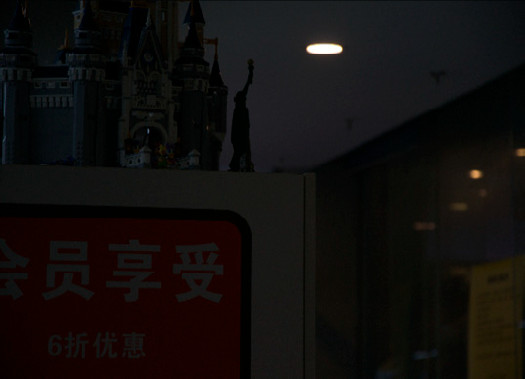
\includegraphics[width=\linewidth]{picture/LLIE/VE-LOL-L/input}
%%				\captionsetup{font=scriptsize}
%%				\caption*{input \\ \quad }
%%				\label{fig: input}
%%			\end{subfigure}
%%			\begin{subfigure}{0.17\columnwidth}
%%				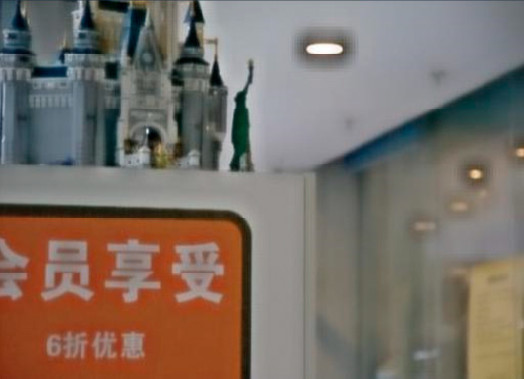
\includegraphics[width=\linewidth]{picture/LLIE/VE-LOL-L/LLNet}
%%				\captionsetup{font=scriptsize}
%%				\caption*{LLNet \\ (2017)}
%%				\label{fig: LLNet_VE_LOL}	
%%			\end{subfigure}
%%			\begin{subfigure}{0.17\columnwidth}
%%				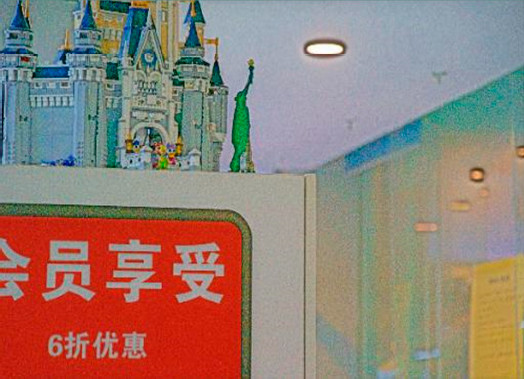
\includegraphics[width=\linewidth]{picture/LLIE/VE-LOL-L/RetinexNet}
%%				\captionsetup{font=scriptsize}
%%				\caption*{RetinexNet \\ (2018)}
%%				\label{fig: RetinexNet_VE_LOL}	
%%			\end{subfigure}
%%			\begin{subfigure}{0.17\columnwidth}
%%				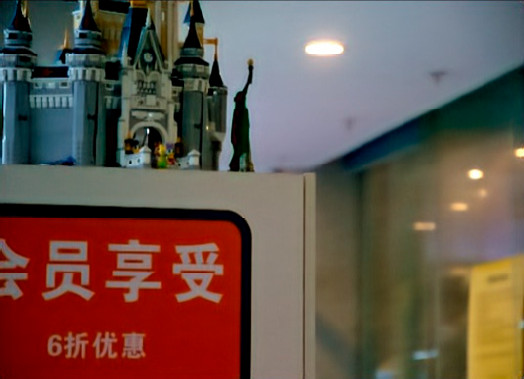
\includegraphics[width=\linewidth]{picture/LLIE/VE-LOL-L/MBLLEN}
%%				\captionsetup{font=scriptsize}
%%				\caption*{MBLLEN \\ (2018)}
%%				\label{fig: MBLLEN_LOL}	
%%			\end{subfigure}
%%			\begin{subfigure}{0.17\columnwidth}
%%				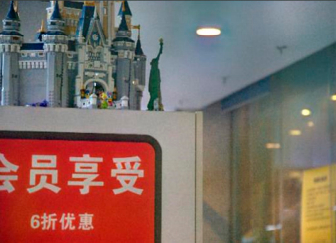
\includegraphics[width=\linewidth]{picture/LLIE/VE-LOL-L/EnlightenGAN}
%%				\captionsetup{font=scriptsize}
%%				\caption*{EnlightenGAN \\ (2019)}
%%				\label{fig: EnlightenGAN_VE_LOL}	
%%			\end{subfigure}
%%			\begin{subfigure}{0.17\columnwidth}
%%				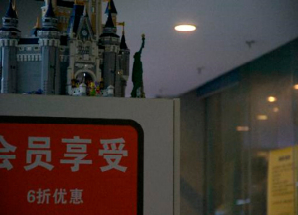
\includegraphics[width=\linewidth]{picture/LLIE/VE-LOL-L/RRDNet}
%%				\captionsetup{font=scriptsize}
%%				\caption*{RRDNet \\ (2020)}
%%				\label{fig: RRDNet_VE_LOL}	
%%			\end{subfigure}
%%			\begin{subfigure}{0.17\columnwidth}
%%				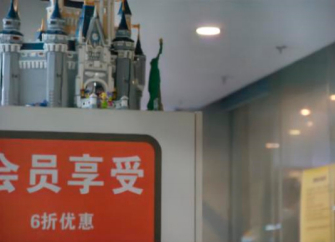
\includegraphics[width=\linewidth]{picture/LLIE/VE-LOL-L/DRBN}
%%				\captionsetup{font=scriptsize}
%%				\caption*{DRBN \\ (2020)}
%%				\label{fig: DRBN_VE_LOL}	
%%			\end{subfigure}
%%			\begin{subfigure}{0.17\columnwidth}
%%				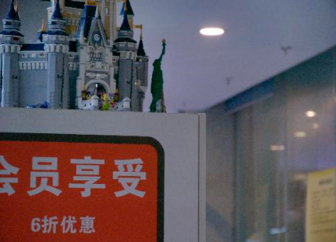
\includegraphics[width=\linewidth]{picture/LLIE/VE-LOL-L/Zero-DCE++}
%%				\captionsetup{font=scriptsize}
%%				\caption*{Zero-DCE++ \\ (2021)}
%%				\label{fig: Zero-DCE++}	
%%			\end{subfigure}
%%			\begin{subfigure}{0.17\columnwidth}
%%				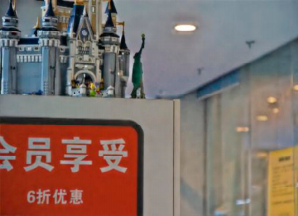
\includegraphics[width=\linewidth]{picture/LLIE/VE-LOL-L/KinD++}
%%				\captionsetup{font=scriptsize}
%%				\caption*{KinD++ \\ (2021)}
%%				\label{fig: KinD++}	
%%			\end{subfigure}
%%			\begin{subfigure}{0.17\columnwidth}
%%				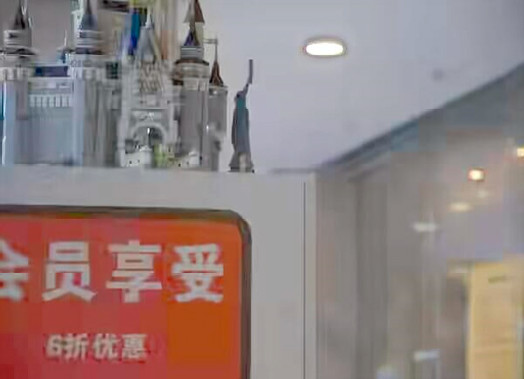
\includegraphics[width=\linewidth]{picture/LLIE/VE-LOL-L/URetinexNet}
%%				\captionsetup{font=scriptsize}
%%				\caption*{URetinexNet \\ (2022)}
%%				\label{fig: URetinexNet}	
%%			\end{subfigure}
%%			\caption{
%%				\label{fig: VE-LOL-L Visual} 
%%				不同算法对从VE-LOL-L 数据集采样的低照度图像的可视化结果。
%%			}
%%		\end{figure}
%		
%		
%		%针对极暗或极亮区域中图像边缘细节恢复的问题,一些研究者提出了在暗区域中加入敏感边缘先验的方法,以降低优化过程中的不适定性,并采用基于编码器-解码器的网络结构和回归损失来执行结构建模。进一步的研究提出了改进的模型,以解决弱光图像中局部边缘失真的问题,并对边缘图与弱恢复图的融合策略进行了优化。
%		
%		本研究提出了三个主要的创新点:(\textcolor{blue}{若并行架构未实现或性能不佳,则可尝试仅通过CNN分支进行图像的弱光恢复,并相应调整创新点,去除并行架构这一创新点。})
%		\begin{itemize}
%			\item[$\bullet$]
%			%首先,提出了一种结合 CNN 和 Transformer 的并行架构用于弱光图像增强。我们发现卷积网络通过合理的增加感受野大小,可以有效捕获图像的局部特征,因而我们利用 UNet 网络对弱光图像进行弱恢复,使用 Swin Transformer 块捕获图像的长距离特征,最后通过特征融合块将二者特征加以融合。
%			
%			首先,提出了一种结合卷积神经网络(CNN)和Transformer的并行架构用于弱光图像增强。在该架构中,UNet网络用于捕获图像的局部特征并进行初步恢复,而Swin Transformer块用于捕获图像的长距离特征。最后,通过特征融合块将两者的特征进行融合,以实现更全面的图像增强效果。
%			\item[$\bullet$] 
%			%其次,在CNN分支中,提出了一个深度语义模块,融合 Swin Transformer 分支,能有效捕获图像长距离特征;
%			其次,提出了一个深度语义模块,该模块融合了Swin Transformer分支,使CNN分支能够有效捕获图像的长距离特征。这种设计增强了CNN分支的能力,使其能够更好地理解图像的全局上下文信息。
%			\item[$\bullet$]
%			%最后,我们将深度可分离卷积融合进 CNN 分支中,应用于轻量级网络用于提取图像的局部特征;
%			最后,将深度可分离卷积融合进CNN分支中,应用于轻量级网络用于提取图像的局部特征。这种设计旨在减少模型的参数量和计算复杂度,同时保持对局部特征的有效提取能力。
%		\end{itemize}
%		
%		\section{实验计划}
%
%		实验的过程中,确保所有的实验在相同的硬件和软件环境下进行,并且为了确保结果的可靠性,可能需要多次运行实验并取平均值。我们主要基于 PyTorch 进行模型的搭建、训练和评估。基于 scikit-image 库计算 PSNR、SSIM 等评价指标。首先构建 U-Net 基本架构模型,然后实现 Swin Transformer 块中的LocalselfAttention类,PositionEncoding类,PositionEmbedding类。
%
%		\subsubsection{Dataset}
%		
%		Tab. \ref{tab: Paired_training_datases} 展示了我们在实验中会使用到的弱光数据集,这些数据集包含真实数据与合成数据。对于每个数据集,我们需要进行如下操作:
%		
%		\begin{itemize}
%			\item [$\bullet$]
%			预处理: 确保所有图像都经过相同的预处理步骤,如尺寸调整、归一化等。
%			
%			\item [$\bullet$]
%			分割: 将每个数据集分为训练集、验证集和测试集。
%		\end{itemize}
%		
%		\begin{table}[!htbp]
%			\centering
%			\tiny
%			%\resizebox{\textwidth}{!}{ %按照宽度调整调整表格大小
%				\begin{tabular}{>{\centering\arraybackslash}m{2.5cm}|c|c|c|c}
%					
%					\hline
%					
%					\textbf{Name} & \textbf{Number} & \textbf{Format} & \textbf{Real/Syn} & \textbf{Video} \\
%					
%					\hline
%					
%					LOL\cite{wei2018deep} & 500 & RGB & Real & \\
%					
%					SCIE\cite{cai2018learning} & 4,413 & RGB & Real & \\
%					
%					VE-LOL-L\cite{jiang2019learning} & 2,500 & RGB & Real+Syn & \\
%					
%					\hline
%					
%				\end{tabular}
%				%}
%			\captionsetup{font=scriptsize} %设置标题字体与表格字体一致
%			\caption{\label{tab: Paired_training_datases}
%				Summary of paired training datasets. 'Syn' represents Synthetic.} %表格的标题
%			
%		\end{table}
%		
%		\subsubsection{Train}
%		
%		\begin{itemize}
%			\item [$\bullet$]
%			基线模型: 首先,训练基线模型。
%			
%			\item [$\bullet$]
%			消融研究: 接着,训练正常 BottleNeck 的模型,以进行消融实验。
%		\end{itemize}
%		
%		\subsubsection{Performance Evaluation}
%		
%		对于每个数据集,使用 Table. \ref{tab: IQA} 指标评估模型性能:
%		
%		\begin{table}[!htbp]
%			\centering
%			\tiny
%			%\resizebox{\textwidth}{!}{ %按照宽度调整调整表格大小
%				\begin{tabular}{>{\centering\arraybackslash}m{5.5cm}|c|c}
%					
%					\hline
%					
%					\textbf{Name} & \textbf{Abbreviation} & \textbf{Reference} \\
%					
%					\hline
%					
%					Peak Signal-to-Noise Ratio                           & PSNR    & \checkmark \\
%					
%					Structural Similarity Index                          & SSIM    & \checkmark \\
%					
%					Learned Perceptual Image Patch Similarity            & LPIPS   & \checkmark \\
%					
%					Multi-Scale Structural Similarity Index              & MS-SSIM & \checkmark \\
%					
%					Mean Squared Error                                   & MSE     & \checkmark \\
%					
%					Mean Absolute Error                                  & MAE     & \checkmark \\
%					
%					Lightness Order Error                                & LOE     & \checkmark \\
%					
%					Blind/Referenceless Image Spatial Quality Evaluator  & BRISQUE & -          \\
%					
%					Neural Image Assessment                              & NIMA    & -          \\
%					
%					Naturalness Image Quality Evaluator                  & NIQE    & -          \\
%					
%					Perceptual Index                                     & PI      & -          \\
%					
%					\hline
%					
%				\end{tabular}
%				%}
%			%\captionsetup{font=scriptsize} %设置标题字体与表格字体一致
%			\caption{
%				\label{tab: IQA}
%				Image quality assessment indicators.} %表格的标题
%			
%		\end{table}
%		
%		\subsubsection{Loss Function}
%		
%		\begin{equation}
%			J_{Huber}(\delta)= \frac{1}{N}\sum_{i=1}^{N}
%			\left\{
%			\begin{aligned}
%				&\frac{1}{2}{\left\|\hat{y}_i - y_i \right\|}_2^{2}, \left\| \hat{y}_i -y_i \right\| < \delta , \\
%				&\delta\left({\left\|\hat{y}_i - y_i \right\|}_1 - \frac{1}{2}\delta \right), \left\| \hat{y}_i -y_i \right\| \geq \delta.
%			\end{aligned}
%			\right.
%			\label{eq: huber loss}
%		\end{equation}
%		
%		\begin{equation}
%			\begin{aligned}
%				\ell_{feat}^{\phi,j} (\hat{y},y) = \frac{1}{C_{j}H_{j}W_{j}}{\left\| \phi_{j}(\hat{y})-\phi_{j}(y)\right\|}_{2}^2
%			\end{aligned}
%			\label{eq: perceptual loss}
%		\end{equation}
%		
%		\begin{equation}
%			\begin{aligned}
%				\mathcal{L}^{\text{SSIM}}(P)=1-\text{SSIM}(\tilde{p}).
%			\end{aligned}
%			\label{eq: revised_SSIM loss}
%		\end{equation}
%		
%		
%		一共尝试以下两种损失函数的搭配方式:
%		
%		\begin{itemize}
%			\item[$\bullet$]
%			休伯损失函数和SSIM损失函数
%			
%			\begin{equation}
%				L_{loss} = \alpha J_{Huber}(\delta) + \beta \mathcal{L}^{\text{SSIM}}(P)
%			\end{equation}
%			
%			\item[$\bullet$]
%			休伯损失函数,SSIM损失函数,Perceptual损失函数(耗费更多训练时间)
%			
%			\begin{equation}
%				L_{loss} = \alpha J_{Huber}(\delta) + \beta \mathcal{L}^{\text{SSIM}}(P) + \gamma \ell_{feat}^{\phi,j} (\hat{y},y)
%			\end{equation}
%		\end{itemize}
		
	\section{实验进度}
		
		\subsection*{已知问题}
		
		\textcolor{red}{低光图像存在严重的噪声、低亮度、低对比度等问题。在以往的研究中,已经提出了多种图像增强方法,但很少有方法能够同时处理这些问题。}\textbf{信息丢失导致的图像细节质量恢复不高}\cite{zhang2023frc}。即当前的深度学习方法增强后的图像仍然存在纹理模糊、光照不准确、色差等问题。几乎所有现有的深度模型都是基于 U-Net 结构,其中包含多个特征缩放操作\cite{ronneberger2015u}。然而,特征缩放不可避免地会失去某些信息视觉原语(Visual primitives)\cite{zhang2021accurate}。特征缩放导致的信息丢失使得增强后的图像丢失了重要的细节,包含了不需要的纹理和颜色。
		
		我们认为目前模型不理想的原因如下:
		
		1) 第一,未能在模型的初始阶段获取更多的图像细节和纹理信息,使得后续的高层次特征处理部分始终停留在图像语义和抽象信息上;
		
		2) 第二,在特征缩放的过程,高级特征虽然深度增加了,但是图像尺寸裁剪使得细节和纹理信息不断丢失,后续在上采样的过程中则放大了这样一种缺失。
		
		3) 第三,使用深度可分离卷积和 ReLU 激活的组合会导致低维流形(Low-dimensional manifolds)上感兴趣信息(Interest information)的丢失\cite{sandler2018mobilenetv2}。
		 
		\textbf{解决第一个问题:}我们尝试以下方法通过增加 Stem 层的深度感知能力,Stem 两个卷积层组成,其中每个层有 64 个 $3 \times 3$ 的过滤器,stride 为1,padding 为1.
		
		\textbf{解决第二个问题:}
		我们尝试引入一种称为自注意蒸馏(Self-attention distillation)的注意模块\cite{guo2019pipeline}以解决上述提到的特征缩放使得图像细节丢失的问题\footnote{\textbf{自注意力蒸馏}(Self-attention distillation): 这是一种注意力机制模块,旨在使低层次特征能够学习高层次特征的语义信息。通过这种方式,可以增强网络的表示学习能力。具体来说,它通过提取不同层次的特征图,并将它们构建为一个自上而下的注意力蒸馏过程,从而实现这一目标。},使得低级特征可以学习到高级特征的语义信息(Semantic information),并通过正则化损失 (Regularization loss) 来约束这一过程,以有效地增强网络的表示学习能力。在自注意蒸馏中,不同层次主干网络中基于激活的(Activation-based)特征图会被提取并构建为自上而下的(Top-down)注意力蒸馏,以增强表示学习过程。具体来说,我们在 U-Net 的编码器网络中添加 Mimic 操作\footnote{Mimic 操作(Mimic operation): 在知识蒸馏 (Knowledge Distillation) 过程中,让一个模型(通常是较小的学生模型)模仿另一个模型(通常是较大的教师模型)的行为或输出。在自注意力蒸馏的上下文中,Mimic 操作指的是让低层次特征模仿高层次特征的行为,以学习更丰富的语义信息。}
		
		除此之外,我们尝试引入FPN(Feature Pyramid Network)\cite{lin2017feature}来处理不同尺度的目标\footnote{FPN(Feature Pyramid Network) 主要包含两个关键步骤:\textbf{自底向上的特征提取}和\textbf{自顶向下的特征融合}。
		\begin{itemize}
			\item [1)]
				自底向上的特征提取阶段通过一个基础网络从输入图像中提取出不同尺度的特征图。这些特征图具有不同的感受野和语义信息。
			
			\item [2)]
				自顶向下的特征融合阶段将高层次特征与低层次特征进行融合,以获得更加丰富和具有多尺度信息的特征表示。\textbf{具体来说,FPN使用上采样操作将较高层级的特征图进行插值得到与相应低层级特征图尺寸相匹配的特征图,然后通过逐元素相加的方式将它们进行融合。}
		\end{itemize}
		
		}。具体而言,我们在 U-Net 网络中的每一个跳跃连接(Skip connection)加入 FPN 模块,采用层层递进的策略,尽可能的减少特征图下采样带来的特征损失。
		
		\textbf{解决第三个问题:}我们需要使用一个称为线性瓶颈(Linear bottlenecks)和反向残差(Inverted residuals)的基本模块来构建编码器网络, 基本模块如Fig. \ref{fig: Base module} 所示,使用激活函数为ReLU6\footnote{
		\begin{equation*}
			f(x) = \min \left( \max \left(0, x\right), 6\right)
		\end{equation*}
		ReLU6 是 ReLU(Rectified Linear Unit)激活函数的变种。其将所有负数的输入值设为 0,并且将所有大于 6 的输入值设为 6。因此,ReLU6 的输出值的范围是 $\left[0, 6\right]$。}
		
		\begin{figure}[htbp]
			\centering
				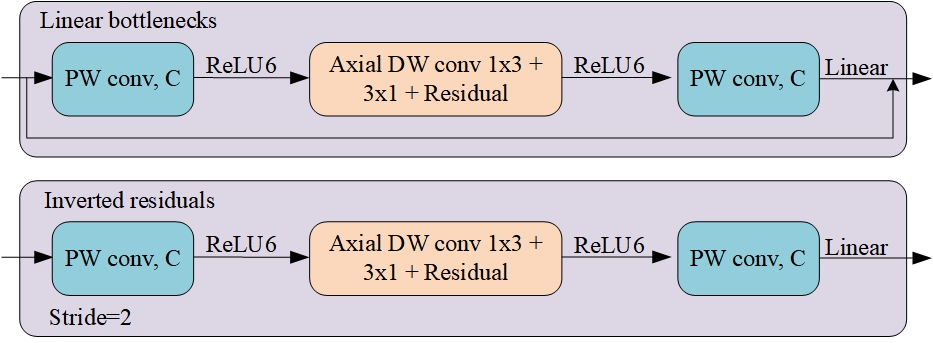
\includegraphics[width=0.7\linewidth]{picture/LLIE/My Architecture/Base module}
				%\captionsetup{font=scriptsize}
				\caption{Linear bottlenecks 和 Inverted residuals}
				\label{fig: Base module}	
		\end{figure}

		\subsection*{实验部分}
		
		如 Fig. \ref{fig: myplot_different_color_channels_low00010}, Fig. \ref{fig: myplot_different_color_channels_low00747}, Fig. \ref{fig: myplot_different_color_channels_low00776}所示, 我们观察到在 Y/Cb/Cr 色彩空间中,Y 通道并不总是能有效地表现出足够的亮度信息。相对而言,在 H/S/V 色彩空间中,H 和 S 通道似乎能更一致地揭示出图像的纹理和结构信息,特别是在光照极低的情境下。这一发现指示了在处理低照度图像时,选择合适的色彩空间对于保留关键视觉信息至关重要。
		
		\begin{figure}[htbp]
			\centering
			\begin{subfigure}{0.3\textwidth}
				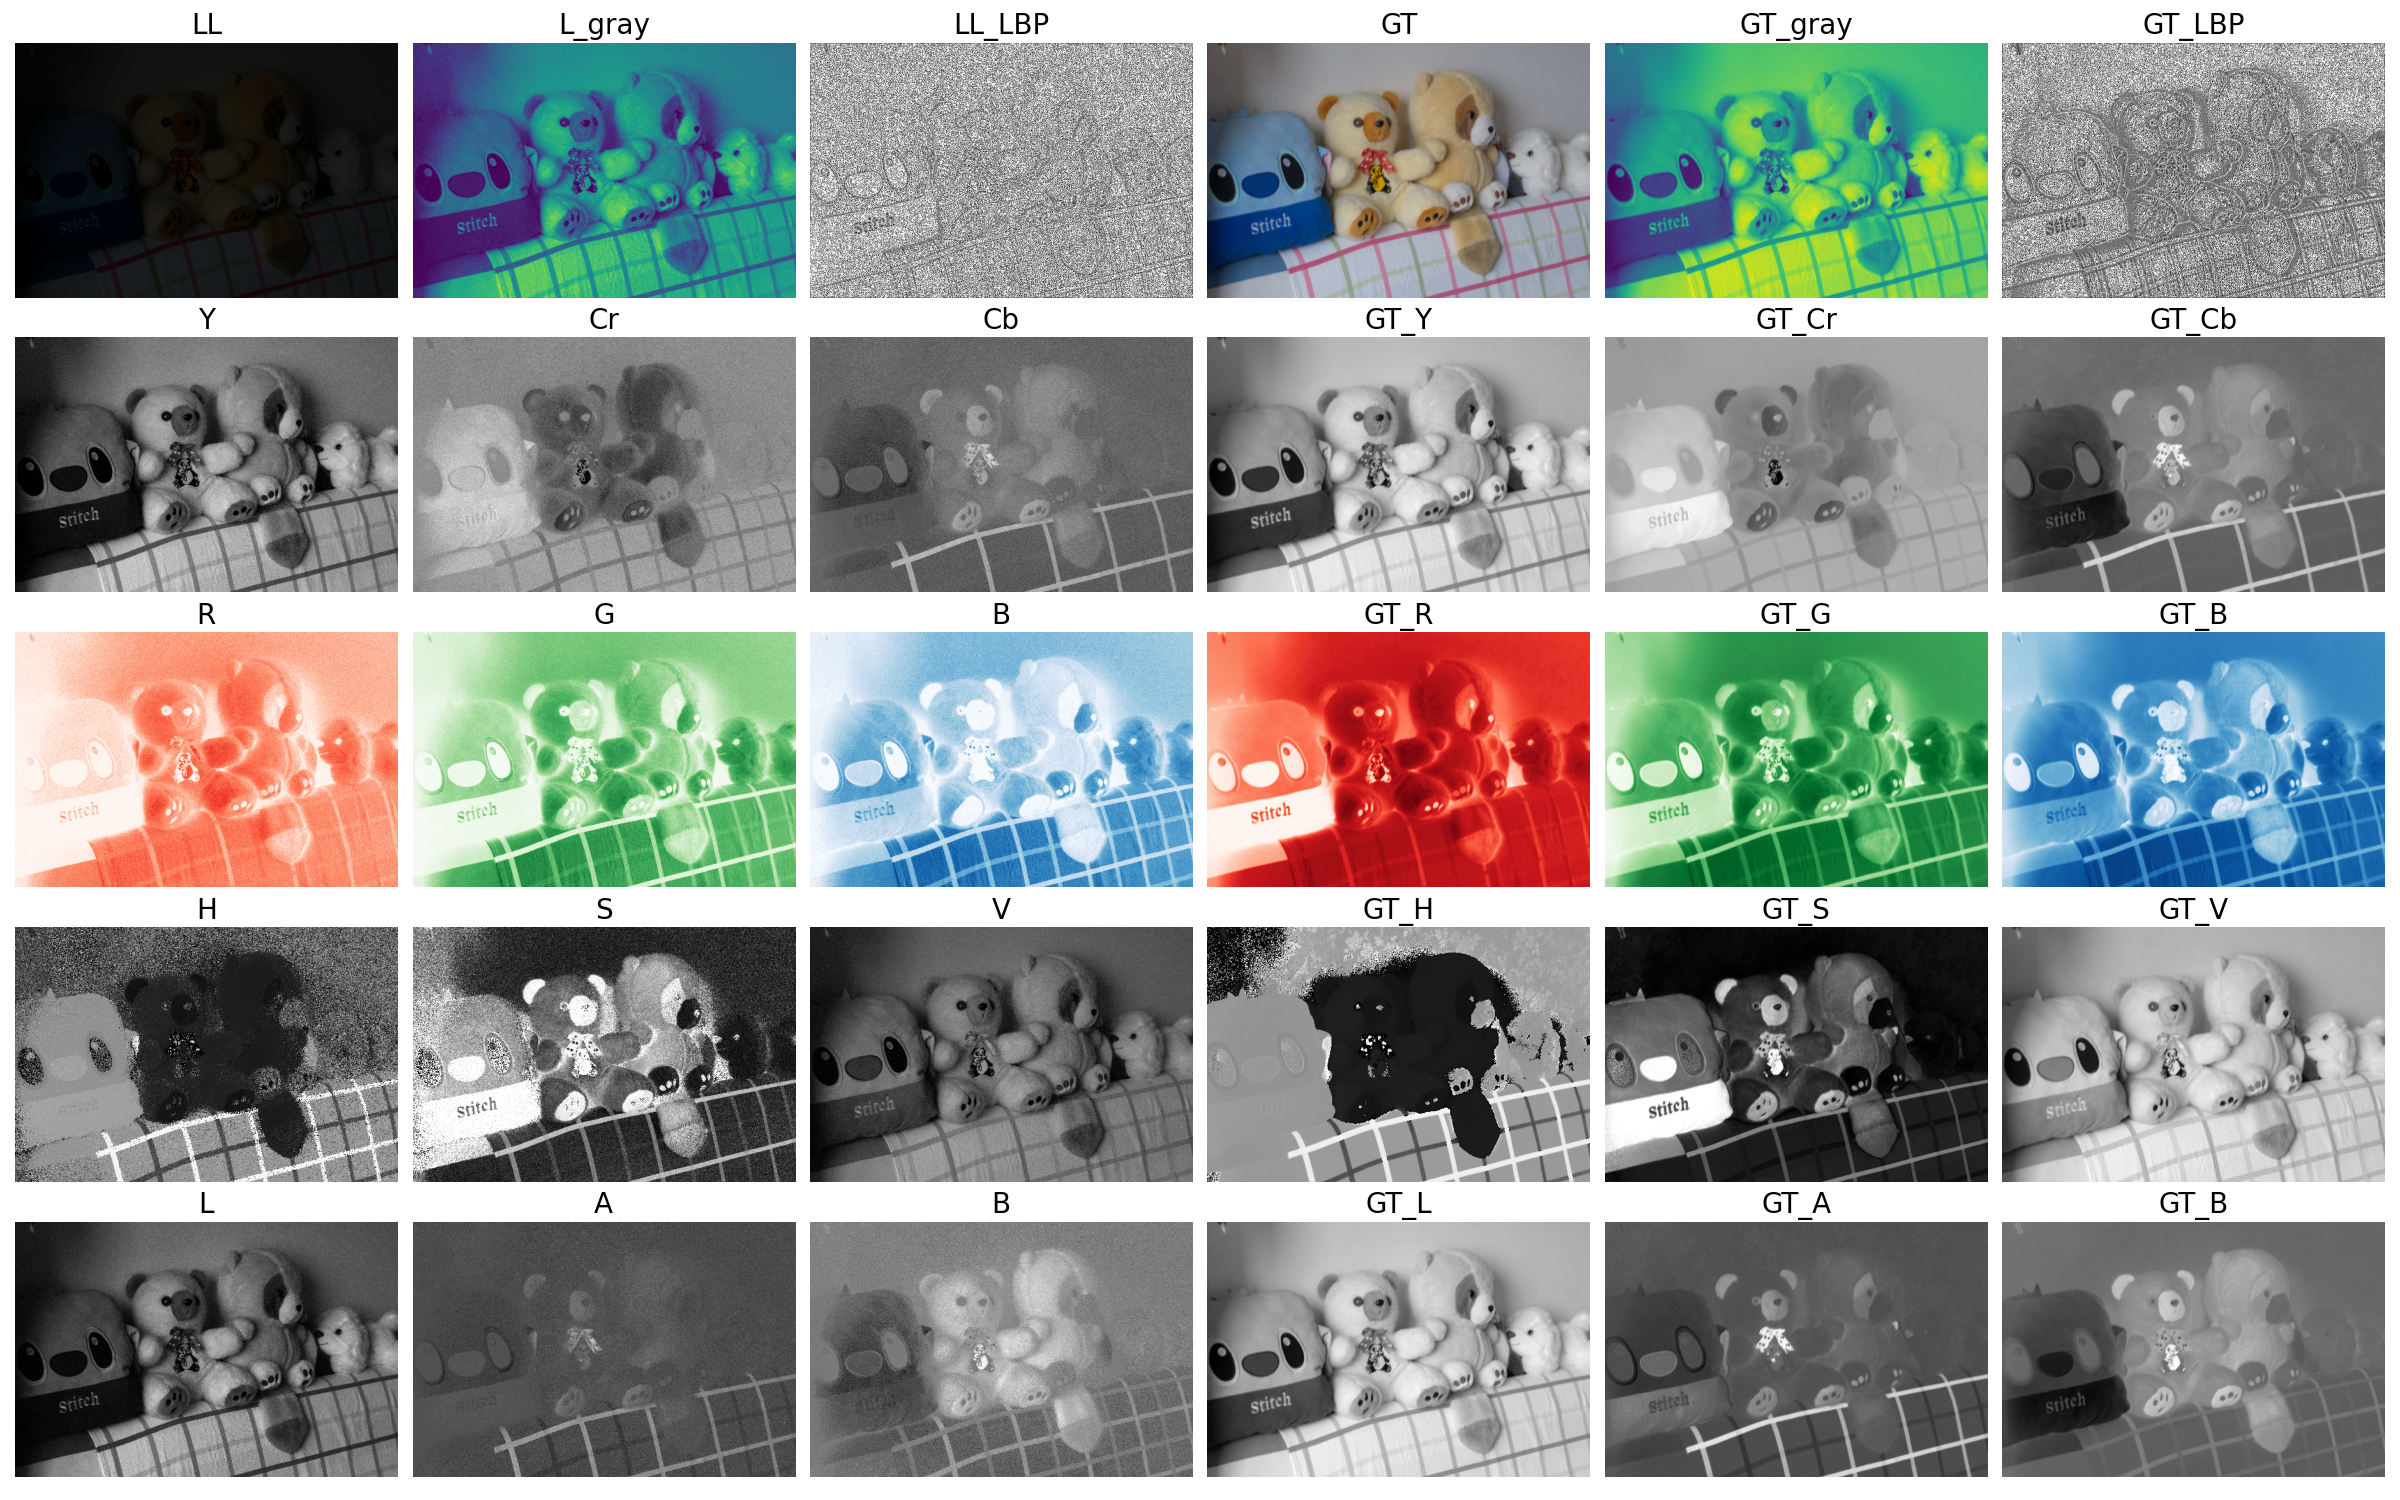
\includegraphics[width=\linewidth]{picture/LLIE/Experiment/myplot_different_color_channels_low00010}
				\captionsetup{font=scriptsize}
				\caption{low00010}
				\label{fig: myplot_different_color_channels_low00010}	
			\end{subfigure}
			\begin{subfigure}{0.3\textwidth}
				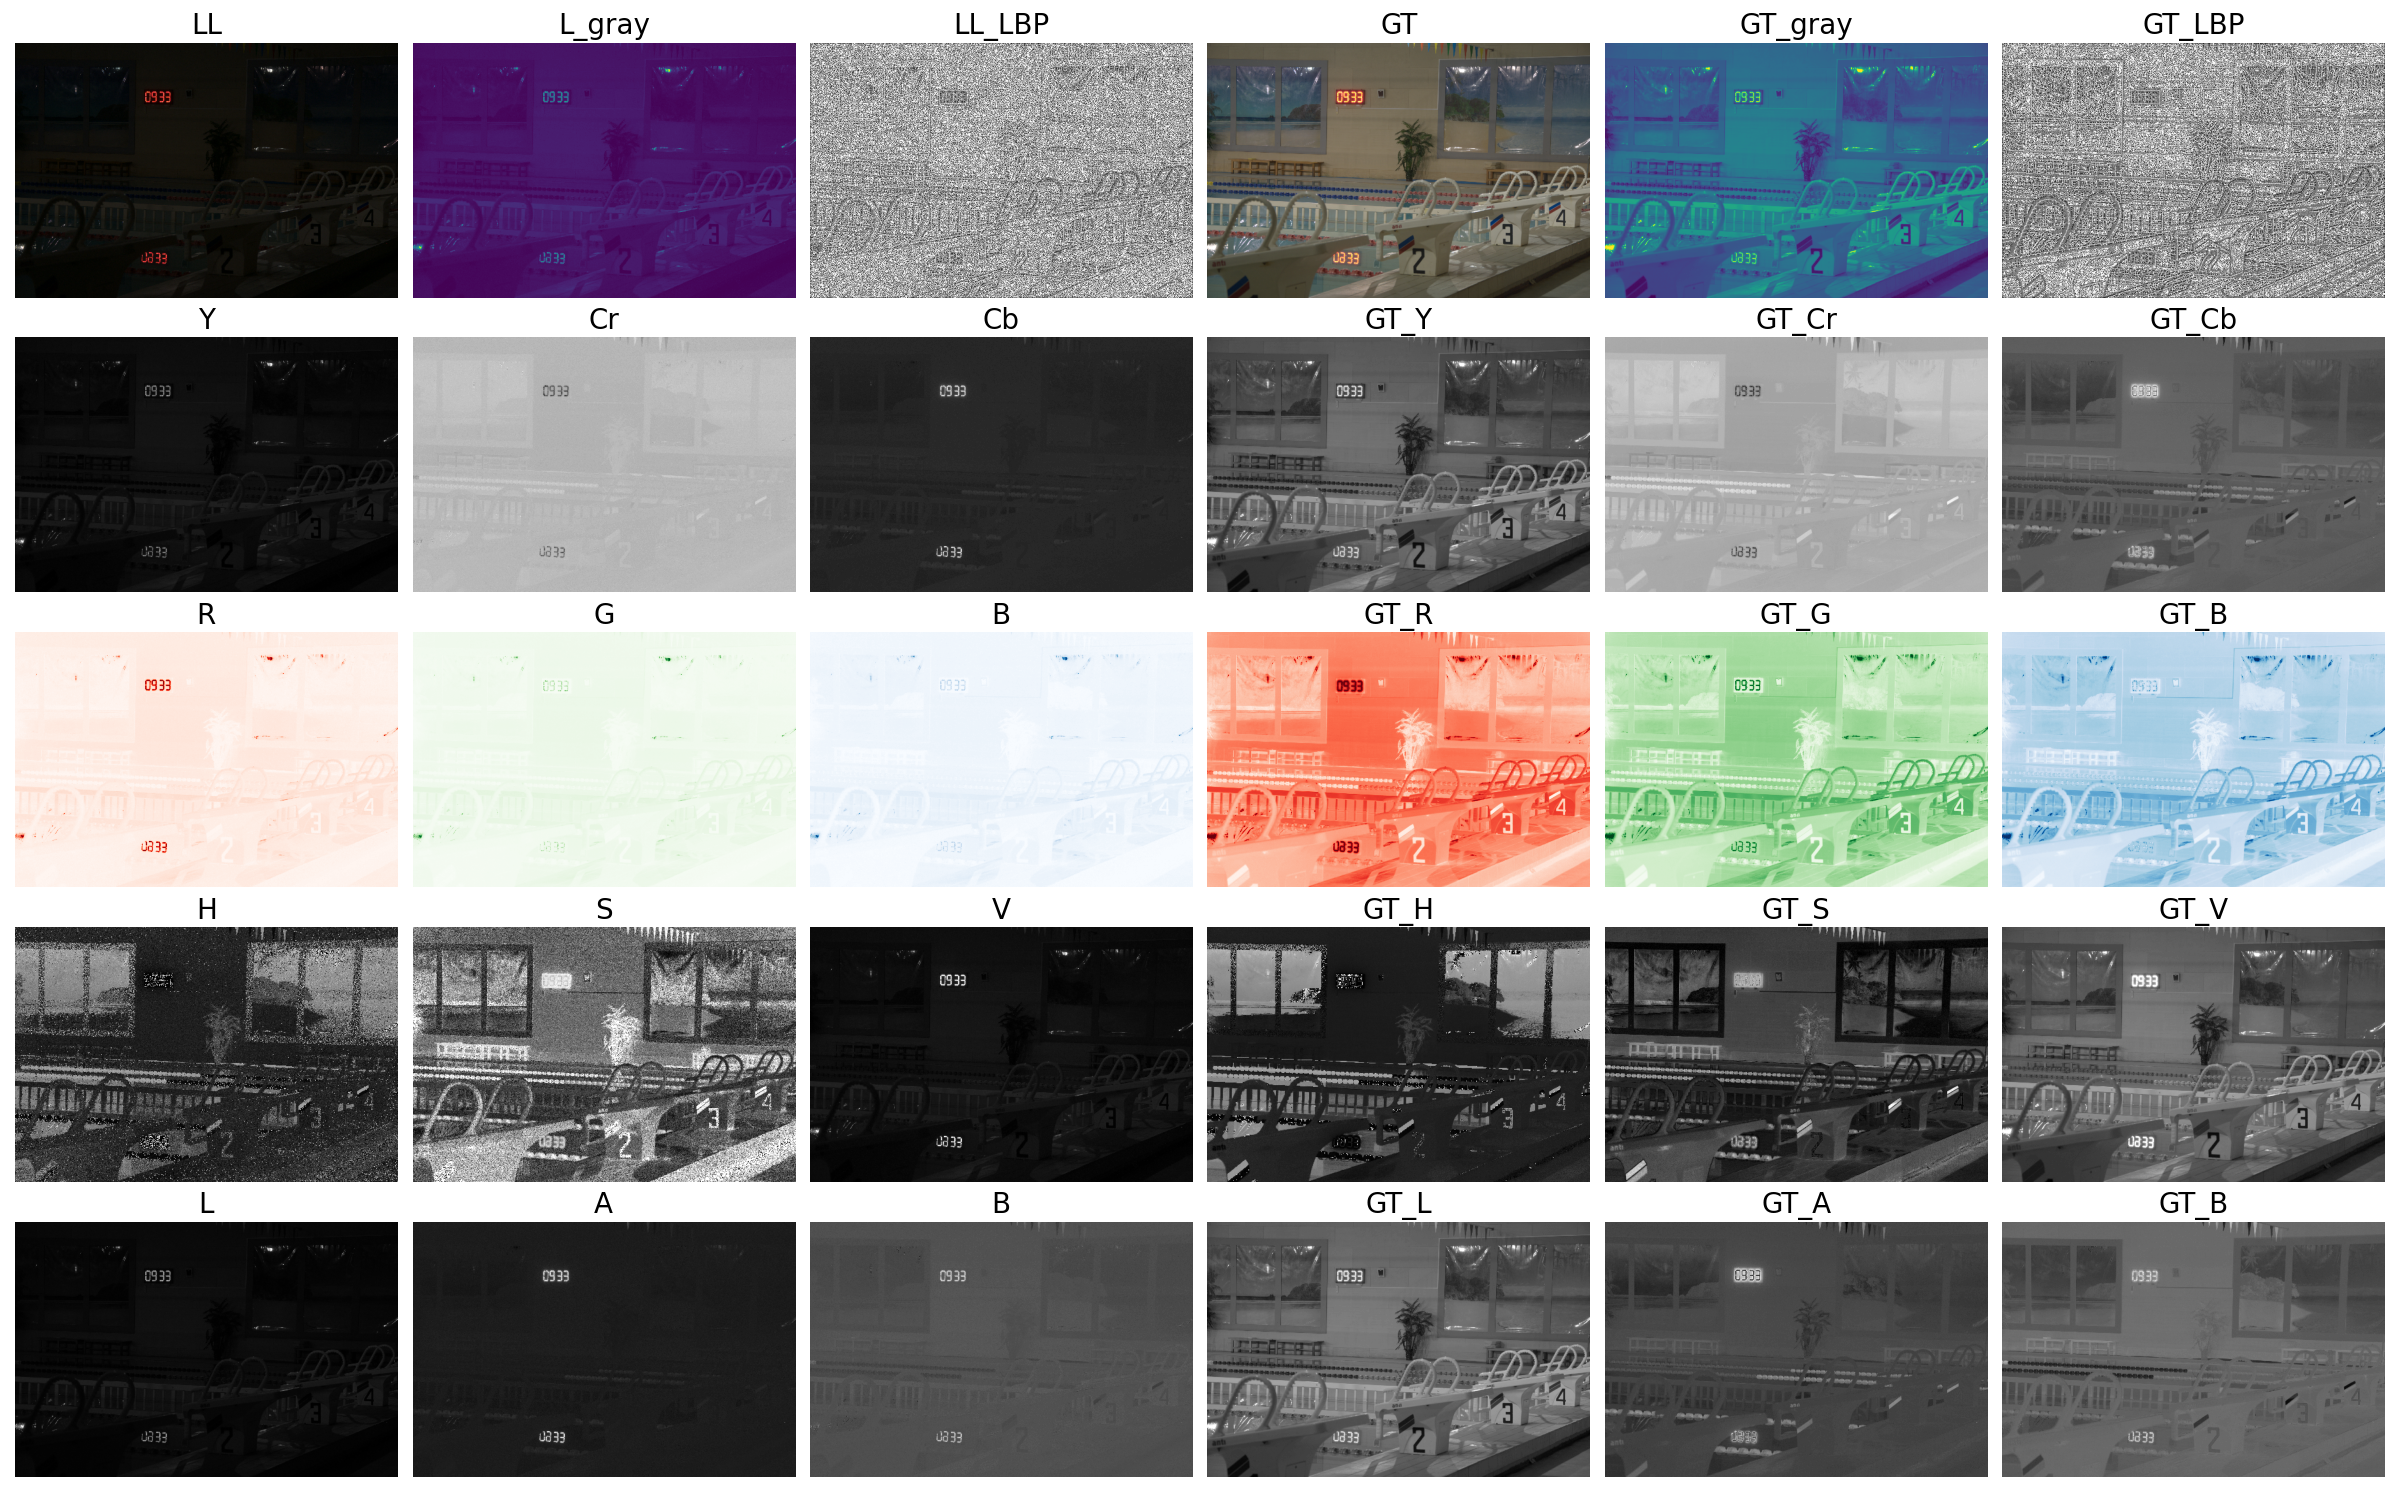
\includegraphics[width=\linewidth]{picture/LLIE/Experiment/myplot_different_color_channels_low00747}
				\captionsetup{font=scriptsize}
				\caption{low00747}
				\label{fig: myplot_different_color_channels_low00747}	
			\end{subfigure}
			\begin{subfigure}{0.3\textwidth}
				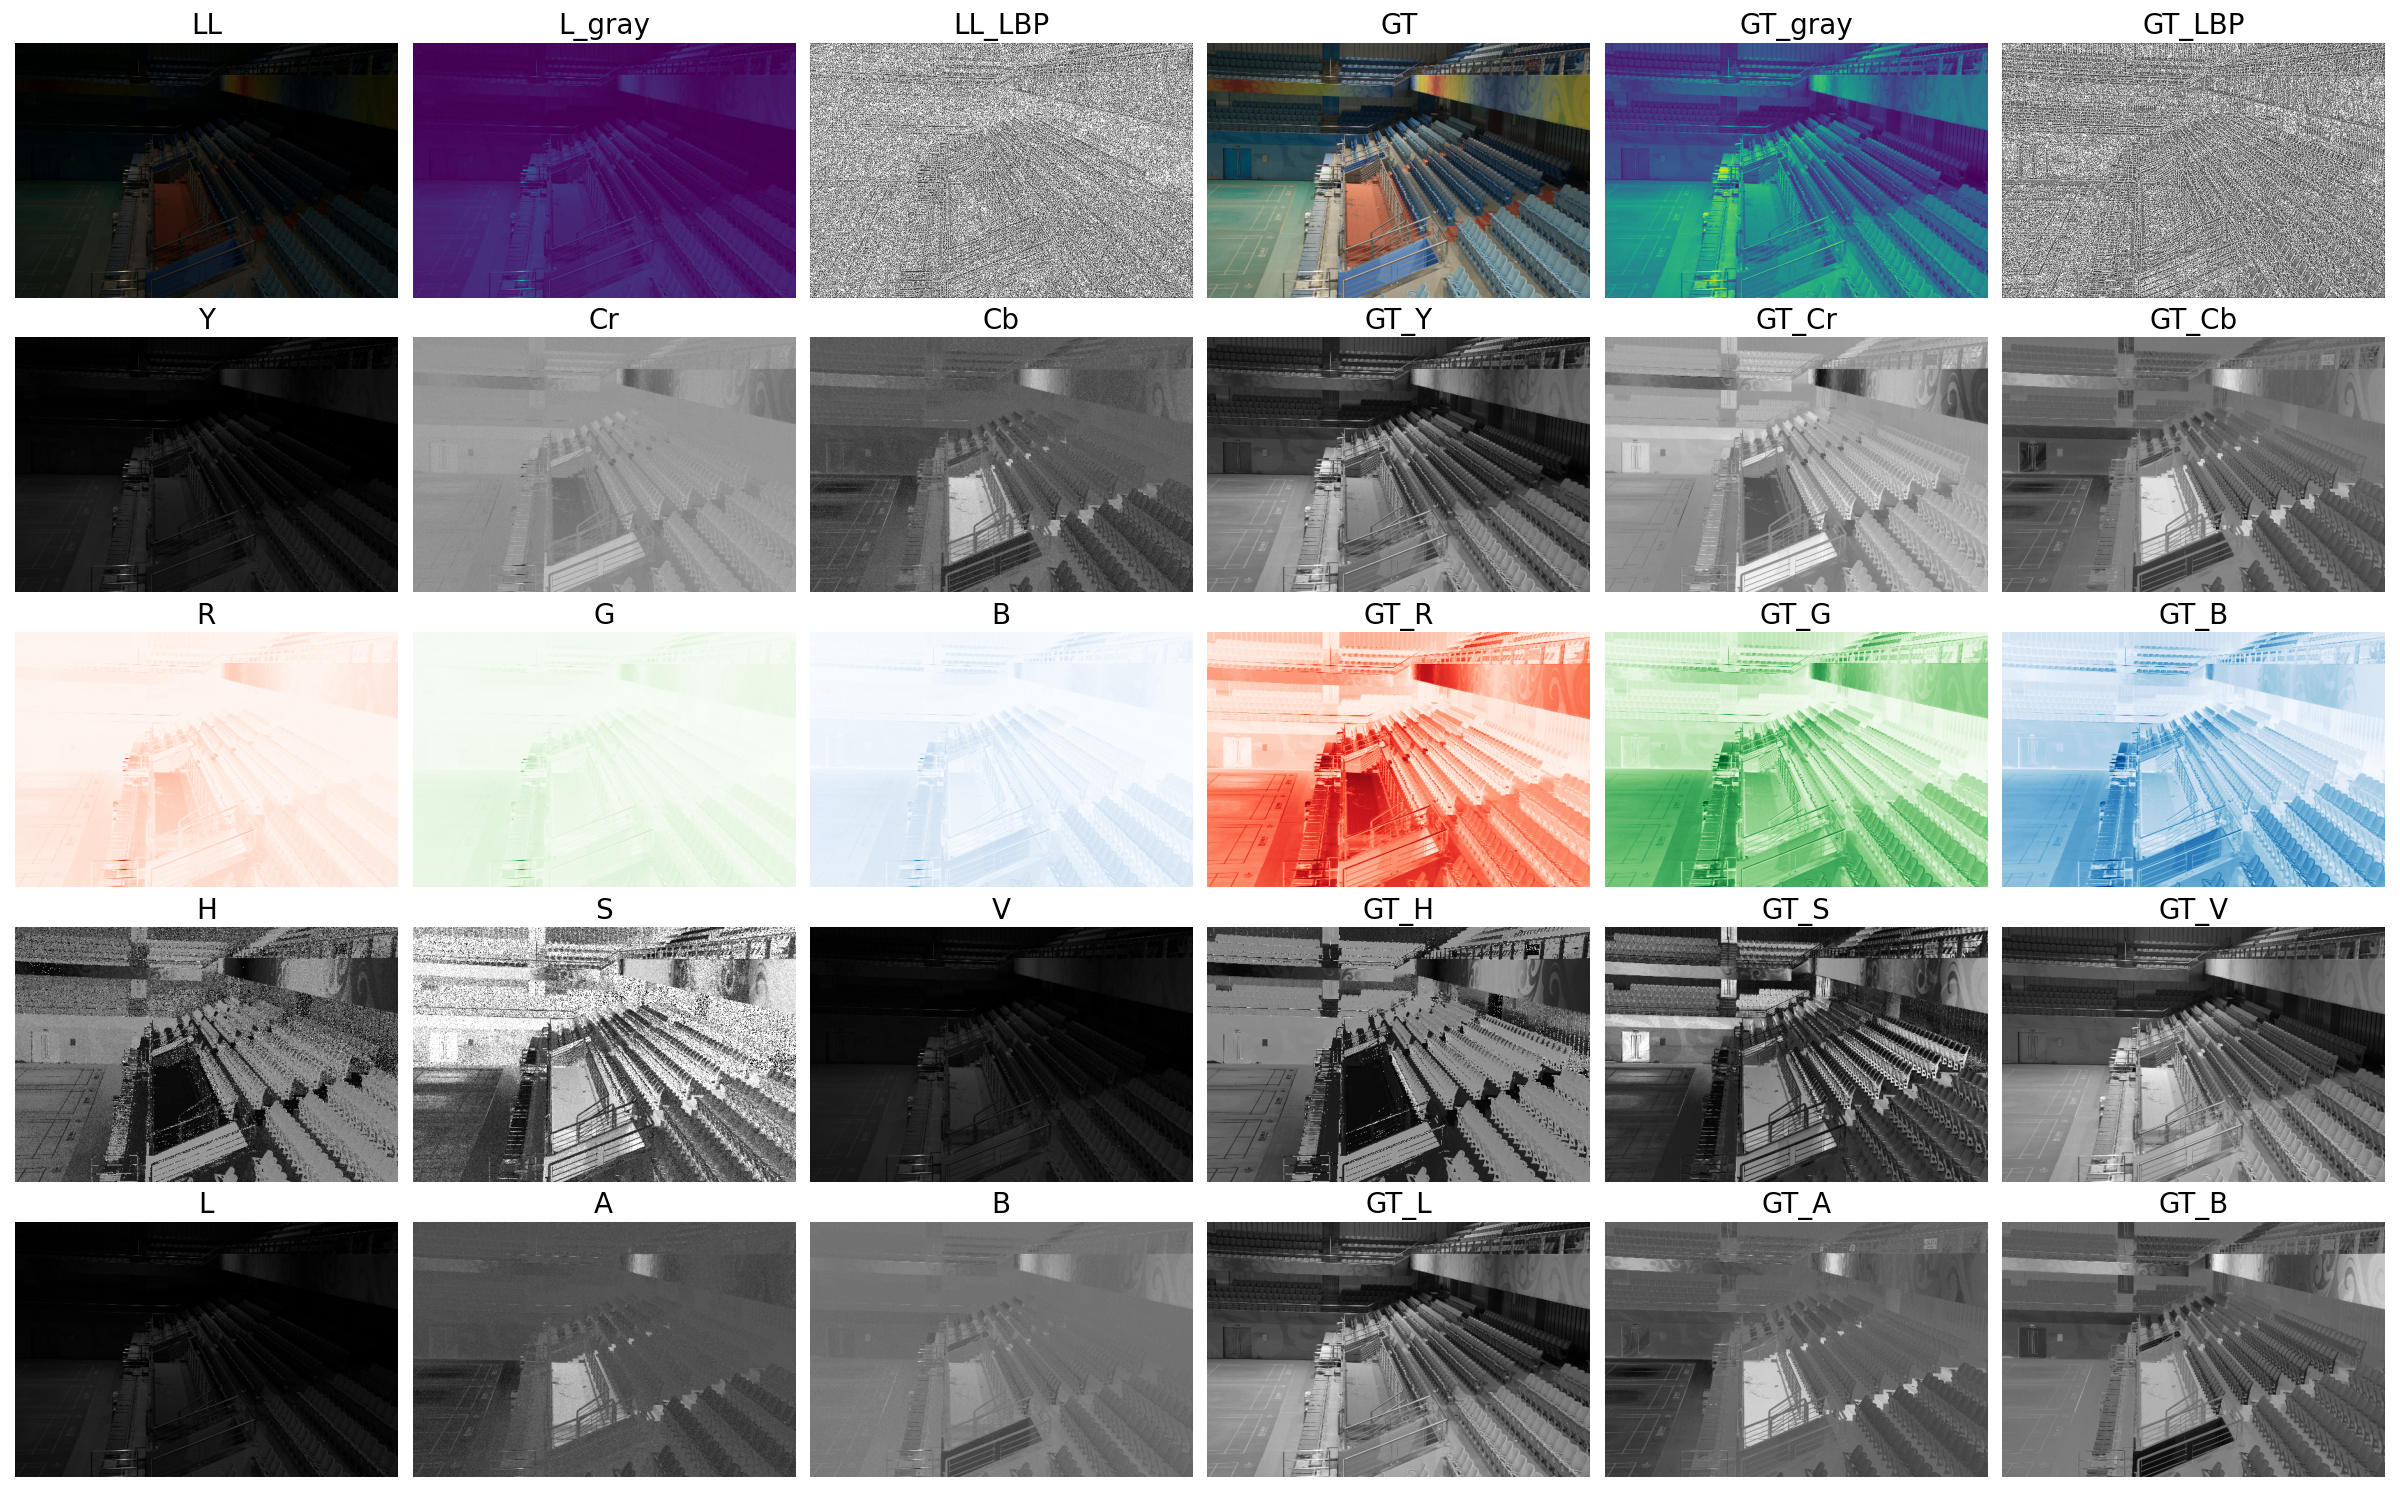
\includegraphics[width=\linewidth]{picture/LLIE/Experiment/myplot_different_color_channels_low00776}
				\captionsetup{font=scriptsize}
				\caption{low00776}
				\label{fig: myplot_different_color_channels_low00776}	
			\end{subfigure}
		\end{figure}
		
		\FloatBarrier
		
		在Fig. \ref{fig: myplot_different_color_channels_low00010}中展示的 low00010 图像分析中,我们可以观察到弱光条件下的RGB通道图片已经相对清晰。对应的 GT 图片主要显示了颜色的加深。此外,通过比较弱光图像与 GT 图像的 Y 通道,我们可以发现亮度特征得到了良好的体现。然而,在 low00747 和 low00776 图像中,如Fig. \ref{fig: myplot_different_color_channels_low00747}和Fig. \ref{fig: myplot_different_color_channels_low00776}所示,相比于 low00010 图像,这两张图片的RGB通道所提供的信息明显不足以支持有效的图像增强。在这些图像中,Y/Cb/Cr通道的 Y 通道同样未能提供足够的信息以供增强处理。
		
		在人造弱光图像的情况中,这种信息缺失更为明显,如Fig. \ref{fig: myplot_different_color_channels_r097088c1t}、Fig. \ref{fig: myplot_different_color_channels_r141669e5t}和Fig. \ref{fig: myplot_different_color_channels_r145221d9t}所示。这些结果表明,在处理不同的图像数据时,简单的颜色加深或亮度增强可能不足以恢复图像质量,特别是当原始数据在关键通道中缺乏足够信息时。
		
		
		在对 HSV 色彩空间进行研究时,我们特别关注了 H(Hue) 通道(色调)的特性。色调通道的分析表明,它能够有效地揭示图像中的颜色种类。在弱光环境下拍摄的图像中,H 通道不仅保留了颜色信息,而且清晰地展示了颜色的变化,这些变化在此环境下可视作“颜色噪声”。通过细致分析H通道,我们可以更有效地把握图像的纹理特征,并恢复出更接近真实场景的颜色表现。我们似乎通过综合利用色调通道提供的独特颜色识别能力,可以在不同光照条件下实现更精确的颜色复原,从而为低光图像处理提供了一种新的视角和方法论。
		
		\textcolor{red}{S (Saturation)通道表示颜色的纯度或浓度,即色彩的深浅程度。饱和度为 0 表示灰度图像,而饱和度为 1 表示完全饱和的纯色。在某些情况下,饱和度图像可能反映出图片的一些结构信息。饱和度一般反映了像素的颜色纯度或浓度,较高的饱和度意味着颜色更加纯净和饱和,而较低的饱和度则意味着颜色更加灰暗和淡薄。在一些图像中,物体的边界或者纹理部分可能具有较高的饱和度,而背景或者平坦的区域可能具有较低的饱和度。因此,在一些情况下,饱和度图像可能会显示出物体的边界或者纹理信息。但是,并不是所有的图像都能够通过饱和度图像准确地反映出结构信息。在某些情况下,饱和度图像可能会受到光照,色彩分布和摄像机参数等因素的影响,导致其无法准确地反映出图像地结构信息。对于弱光图像来说,饱和度(S)通道通常不能很好地反映出图片地结构信息。弱光图像通常是指光照条件较差或者光照不均匀的图像,在这种情况下,图像的色彩信息可能会受到影响,导致饱和度较低,即使存在一定的色彩变化或者结构信息,也可能无法很好地体现在饱和度通道中。}
					
		\textcolor{red}{V (Value)通道表示颜色的亮度或明暗程度。明度为 0 表示黑色,而明度为 1 表示白色。对于弱光图像来说,亮度(V)通道通常能够更好地反映出图片的结构和纹理信息。亮度通道代表了图像的明暗程度,而在弱光条件下,图像的色彩信息可能会受到影响,导致饱和度和色调较低,即使存在一定的色彩变化或者结构信息,也可能无法很好地体现在饱和度和色调通道中。综上所述,对于弱光图像更适合使用亮度(V)通道来反映图片的结构信息。}
		
		\begin{figure}[htbp]
			\centering
			\begin{subfigure}{0.3\textwidth}
				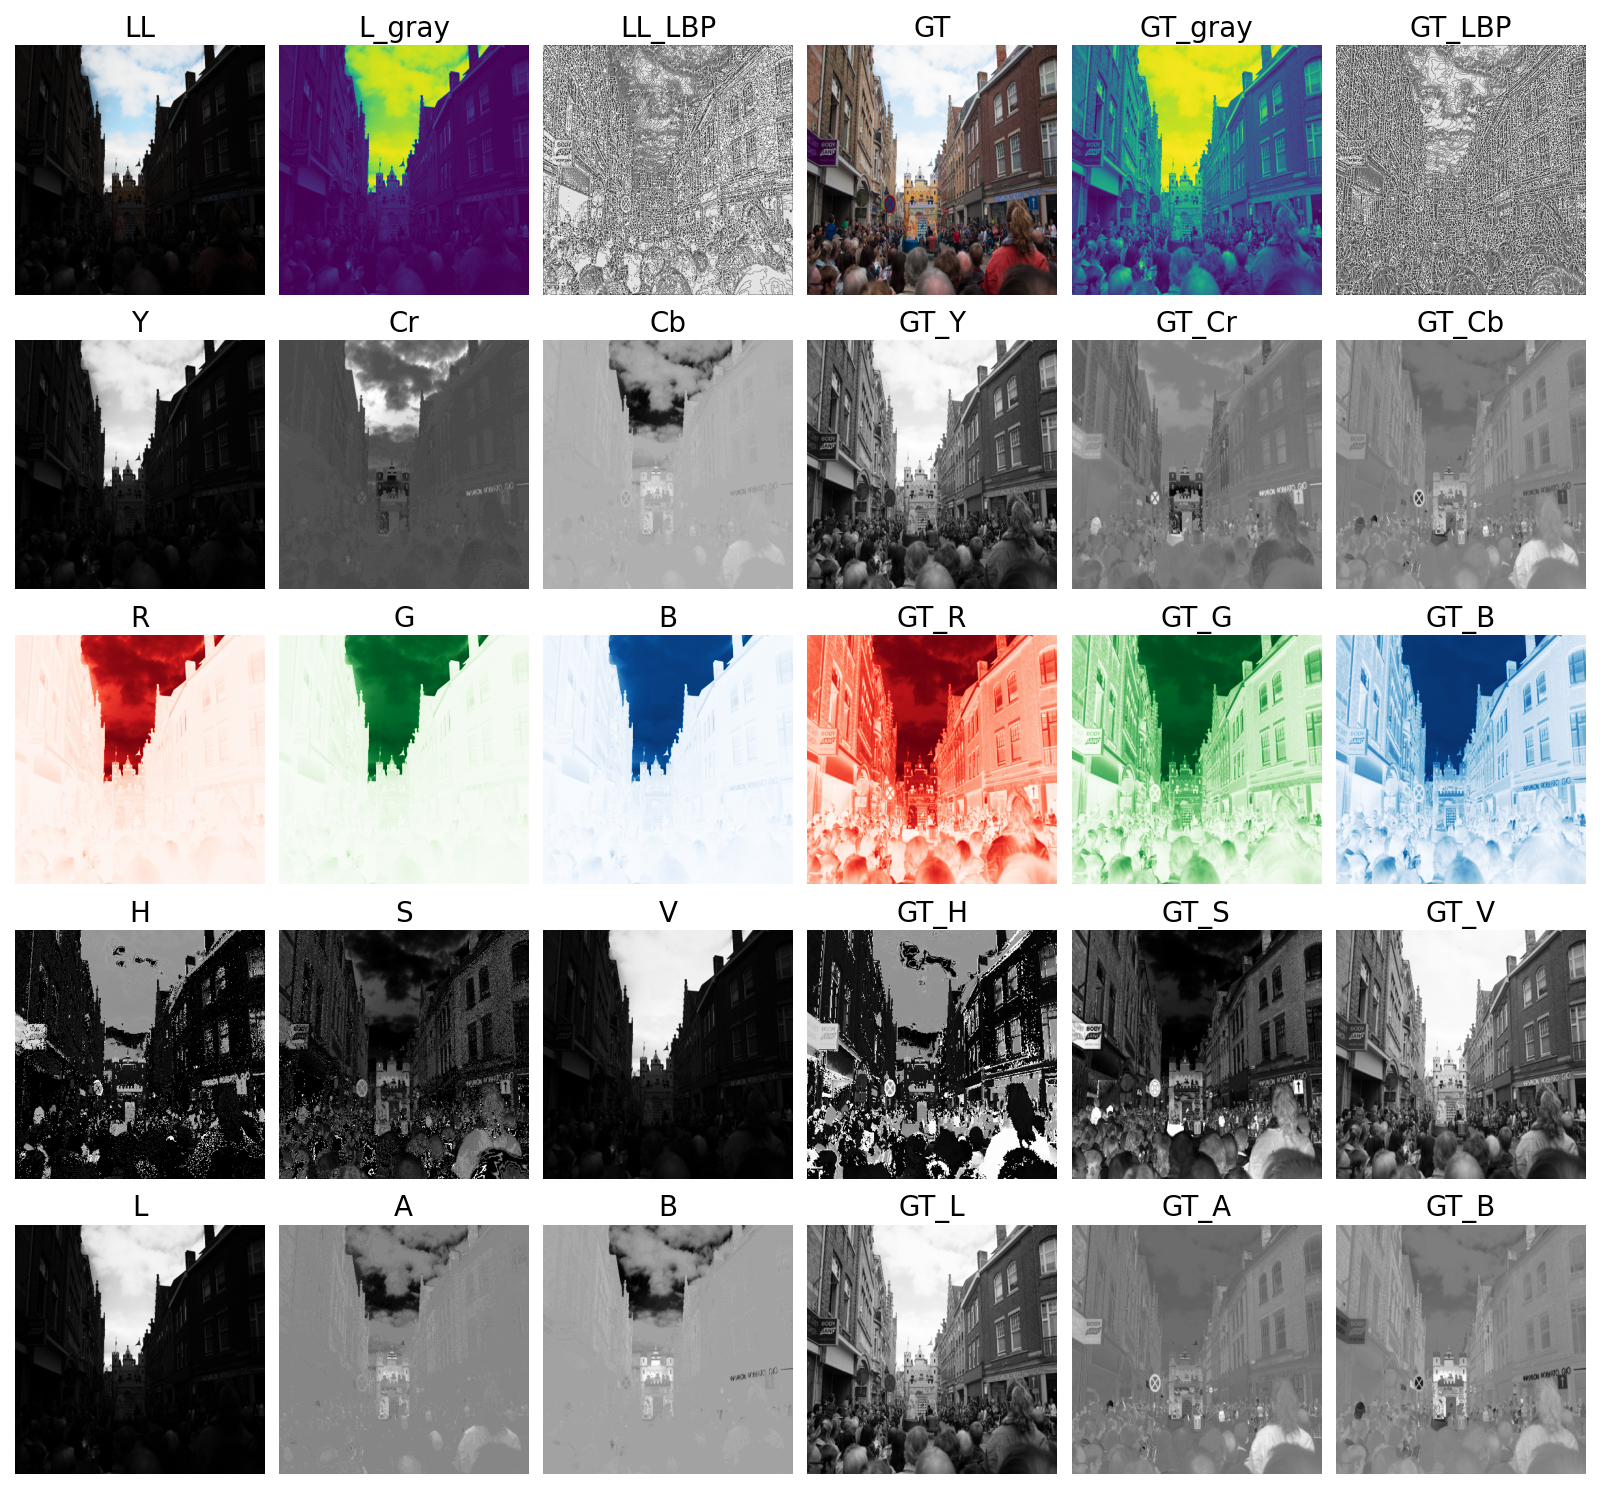
\includegraphics[width=\linewidth]{picture/LLIE/Experiment/myplot_different_color_channels_r097088c1t}
				\captionsetup{font=scriptsize}
				\caption{r097088c1t}
				\label{fig: myplot_different_color_channels_r097088c1t}	
			\end{subfigure}
			\begin{subfigure}{0.3\textwidth}
				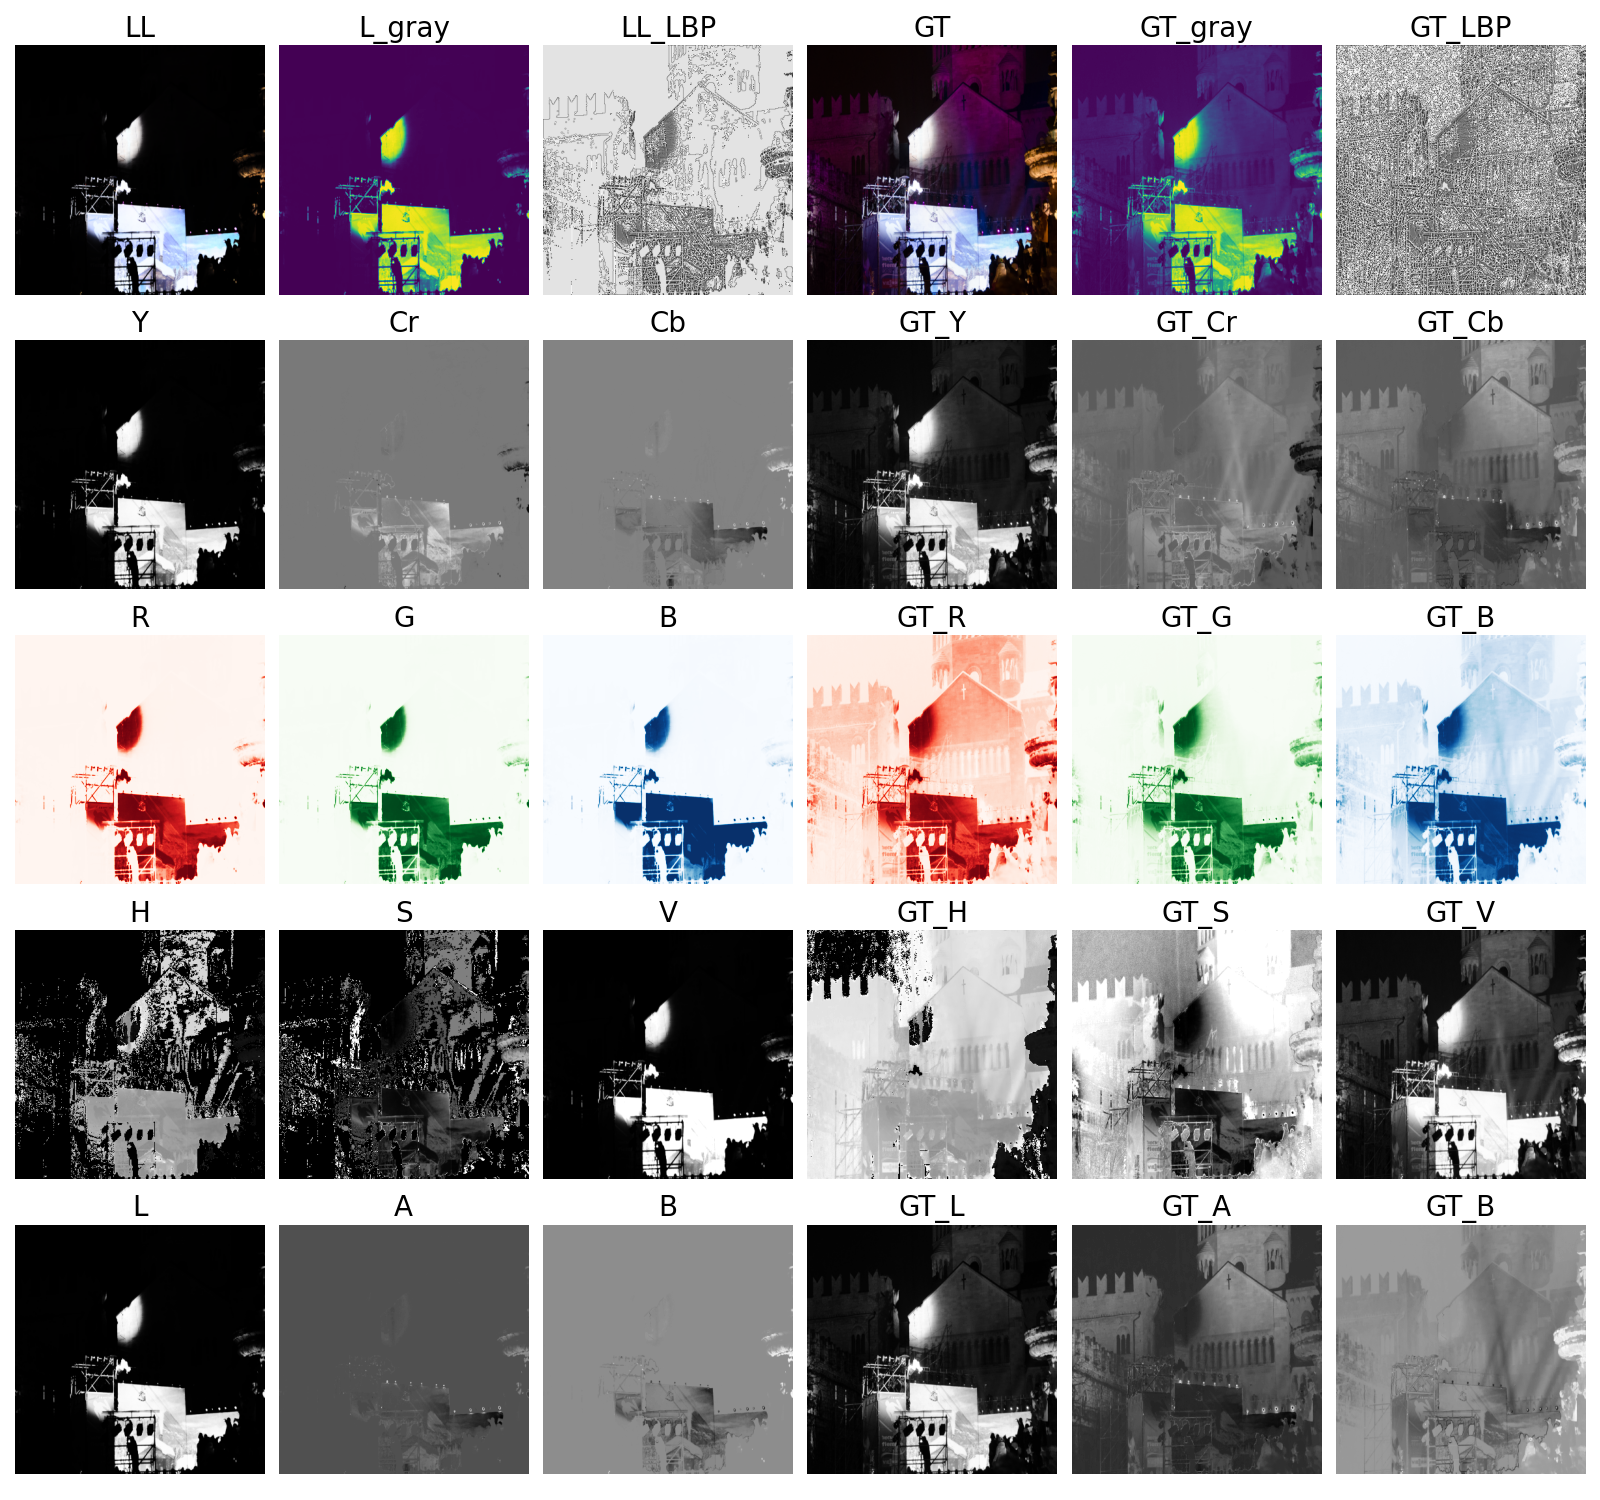
\includegraphics[width=\linewidth]{picture/LLIE/Experiment/myplot_different_color_channels_r141669e5t}
				\captionsetup{font=scriptsize}
				\caption{r141669e5t}
				\label{fig: myplot_different_color_channels_r141669e5t}	
			\end{subfigure}
			\begin{subfigure}{0.3\textwidth}
				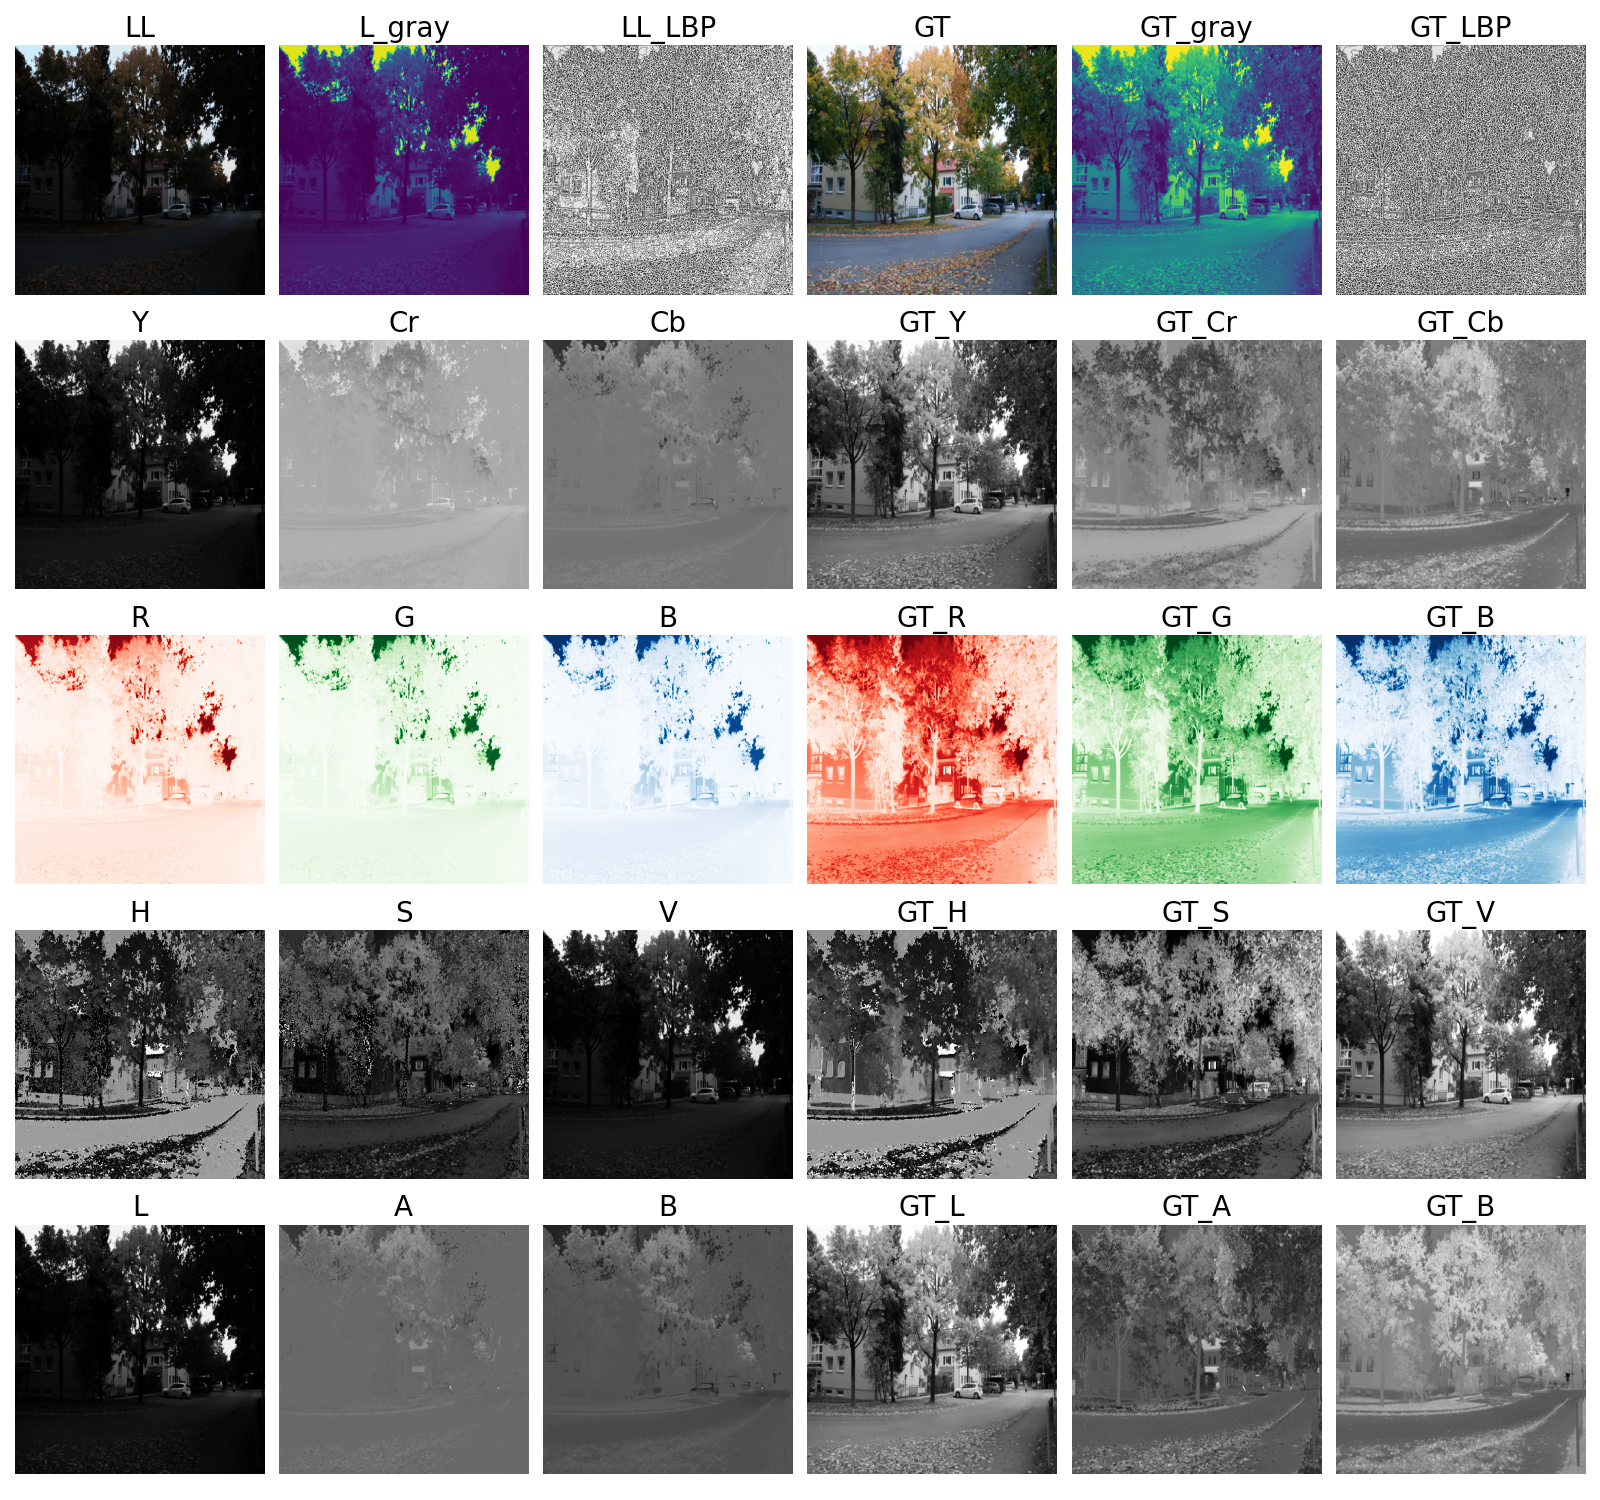
\includegraphics[width=\linewidth]{picture/LLIE/Experiment/myplot_different_color_channels_r145221d9t}
				\captionsetup{font=scriptsize}
				\caption{r145221d9t}
				\label{fig: myplot_different_color_channels_r145221d9t}	
			\end{subfigure}
		\end{figure}
		
		\FloatBarrier
		
		\subsection*{对注意力机制的改进方法}
		
		\subsubsection*{MSAM}
		
		我们将多尺度卷积注意模块 (Multi-scale convolutional attention, MSCA) 引入 CBAM 模块中,使得通道注意力也具备多尺度性能,多分支深度卷积或许可以更好的提取多尺度特征,如 Fig. \ref{fig: MSAM} 所示。
		
		\begin{figure}[htbp]
			\centering
			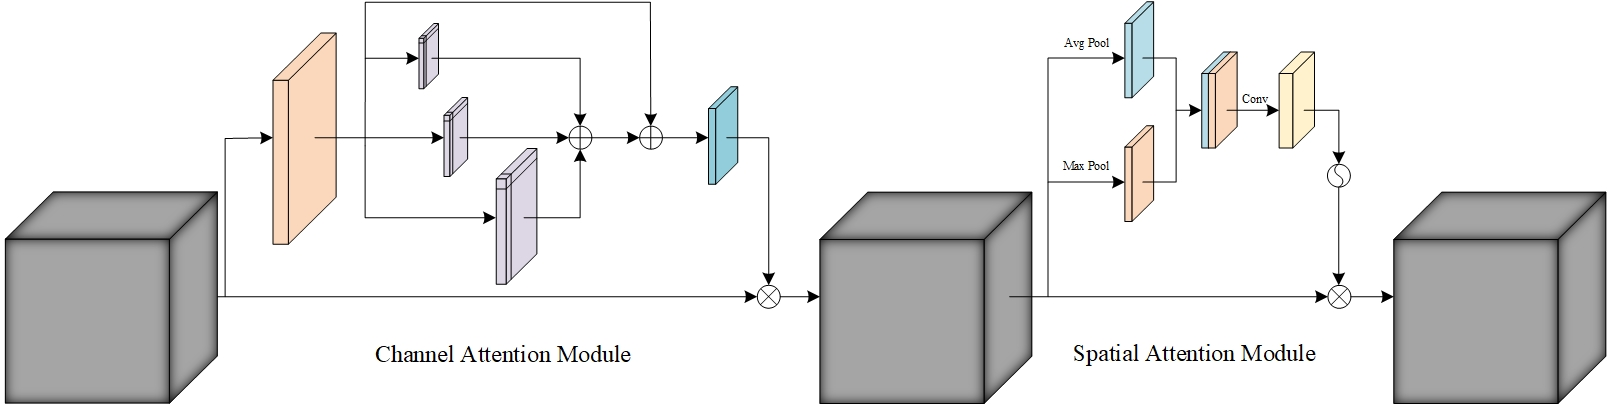
\includegraphics[width=0.8\linewidth]{picture/LLIE/Experiment/Attention/MSAM}
			%\captionsetup{font=scriptsize}
			\caption{MSAM}
			\label{fig: MSAM}
		\end{figure}
		
		具体来说,MSCA 首先通过一个 $5 \times 5$ 的卷积核进行卷积操作,然后分别使用 $7 \times 7$、$11 \times 11$ 和 $21 \times 21$ 的多尺度深度卷积核对特征图进行处理,以捕捉不同尺度的特征信息。接着将这些尺度上的特征图相加,并与输入的残差特征相加,最后通过一个 $1 \times 1$ 的卷积核对通道进行调整,以获得最终的注意力特征表示。
		
		\subsubsection*{CPCS}
		
		SegNeXt 是一种用于语义分割的简单卷积网络体系结构\cite{guo2022segnext},作者通过对已有成功分割方案进行了重新审视,发现了几个有助于性能提升地关键成分,进而促使作者设计了一种新型地卷积注意力架构方案,多尺度卷积注意模块(Multi-scale convolutional attention, MSCA),其原理主要是将 CBAM 块中的通道注意力替换为 MSCA,使通道注意力具备多尺度性能。MSCA块证明了卷积注意比Transformer中的自注意机制更有效地编码上下文信息。
		
		如 Fig. \ref{fig: MSCA} 所示,MSCA包含三个部分:深度卷积聚合局部信息,多分支深度可分离卷积捕获多尺度上下文,以及 $1 \times 1$ 卷积建模不同通道之间的关系。通过采用多尺度深度卷积模块,可以有效地提取空间关系,同时保留通道先验\cite{huang2023channel}。
		
		\begin{figure}[htbp]
			\centering
			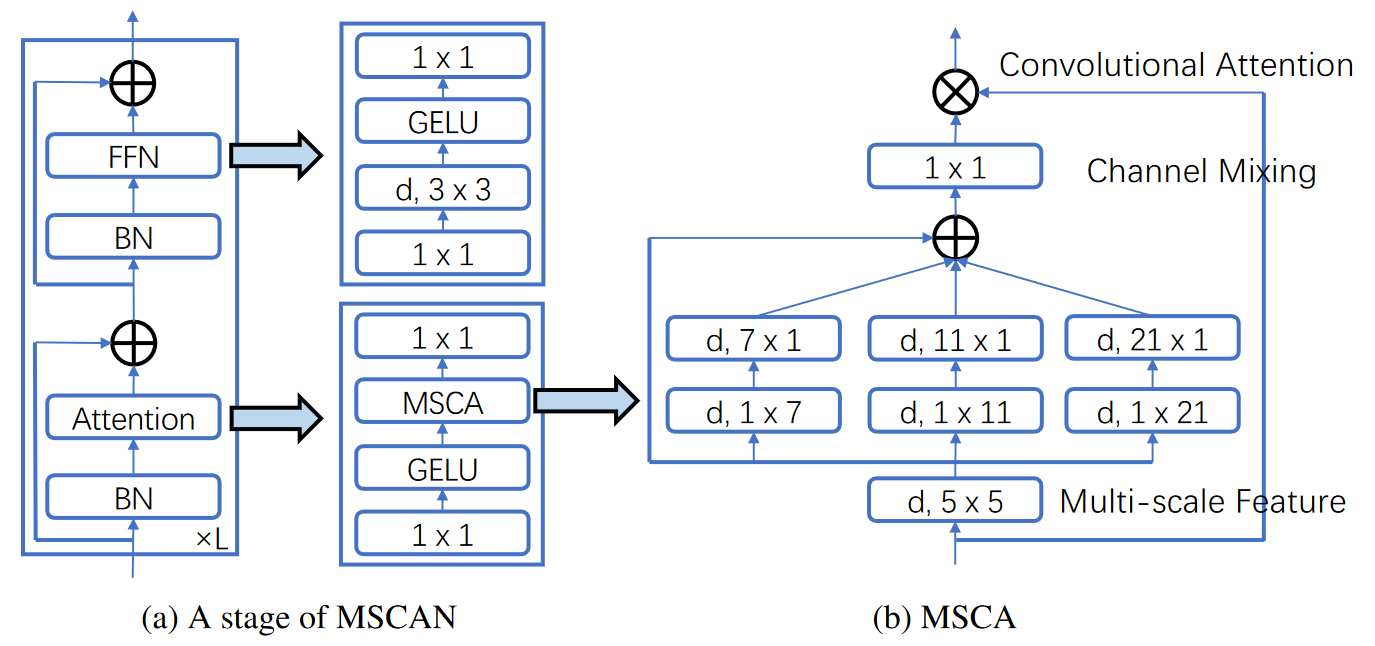
\includegraphics[width=0.8\linewidth]{picture/LLIE/Experiment/Attention/MSCA}
			%\captionsetup{font=scriptsize}
			\caption{MSCA}
			\label{fig: MSCA}
		\end{figure}
			
	 	SE 只整合了通道注意力,这限制了它选择重要区域的能力。CBAM 整合了通道注意力和空间注意力,但它在其输出特征的所有通道上强制执行一致的空间注意力分布。如Fig. \ref{fig: SE_CBAM_CPCA}(c)所示,作者\cite{huang2023channel}提出一种新的通道优先卷积注意力(Channel Prior Convolutional Attention, CPCA)方法,采用多尺度的深度可分离卷积模块构成空间注意力,可以在通道和空间维度上动态分配注意权重。
	 	
	 	\begin{figure}[htbp]
	 		\centering
	 		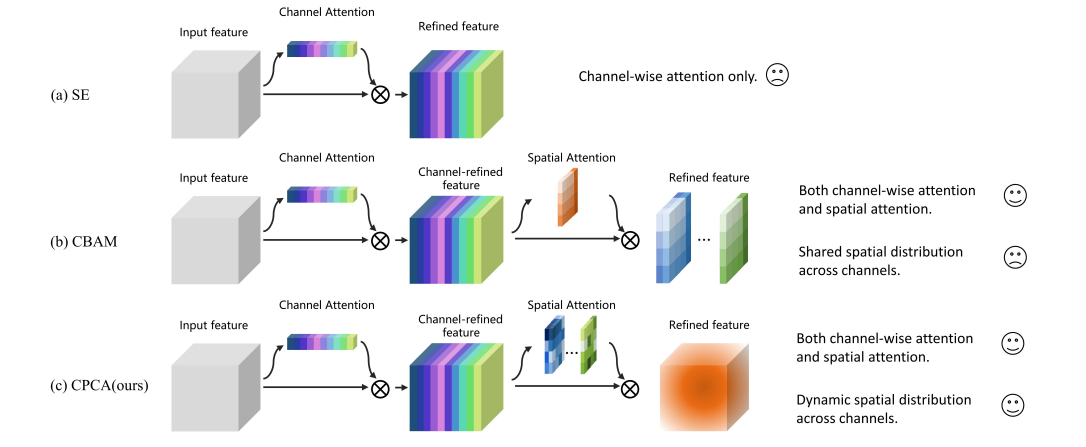
\includegraphics[width=0.8\linewidth]{picture/LLIE/Experiment/Attention/SE_CBAM_CPCA}
	 		%\captionsetup{font=scriptsize}
	 		\caption{Schematic representation of the refined features of the three attention mechanisms (a) SE, (b) CBAM, and (c) CPCA.}
	 		\label{fig: SE_CBAM_CPCA}
	 	\end{figure}
		 
		CPCA的整体结构包括通道注意力和空间注意力的顺序放置。特征图的空间信息是由通道注意力通过平均池化和最大池化等操作来聚合的。随后,空间信息通过共享多层感知器(shared MLP)进行处理并添加以生成通道注意力图。通道先验是通过输入特征和通道注意力图的元素相乘获得的。随后,通道先验被输入到深度卷积模块中以生成空间注意力图。卷积模块接收空间注意力图以进行通道混合。最终,通过通道混合结果与通道先验的逐元素相乘,获得细化的特征作为输出。多尺度深度可分离卷积注意力原理图见Fig. \ref{fig: CPCA}.
		
		\begin{figure}[htbp]
			\centering
			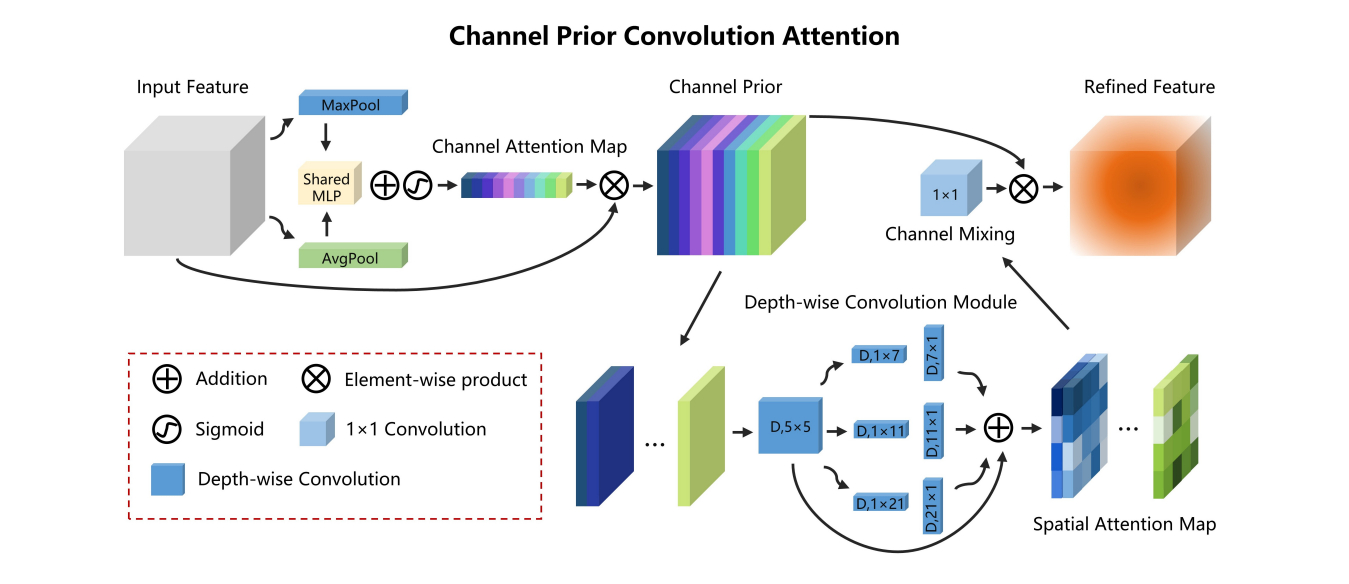
\includegraphics[width=0.8\linewidth]{picture/LLIE/Experiment/Attention/CPCA}
			%\captionsetup{font=scriptsize}
			\caption{CPCA}
			\label{fig: CPCA}
		\end{figure}
		
		我们结合上述两种方法,如 Fig. \ref{fig: CPMS} 所示,设计一种多尺度通道注意力和多尺度深度可分离卷积空间注意力(Channel Prior Multi-Scale Attention, CPMS)
		
		\begin{figure}[htbp]
			\centering
			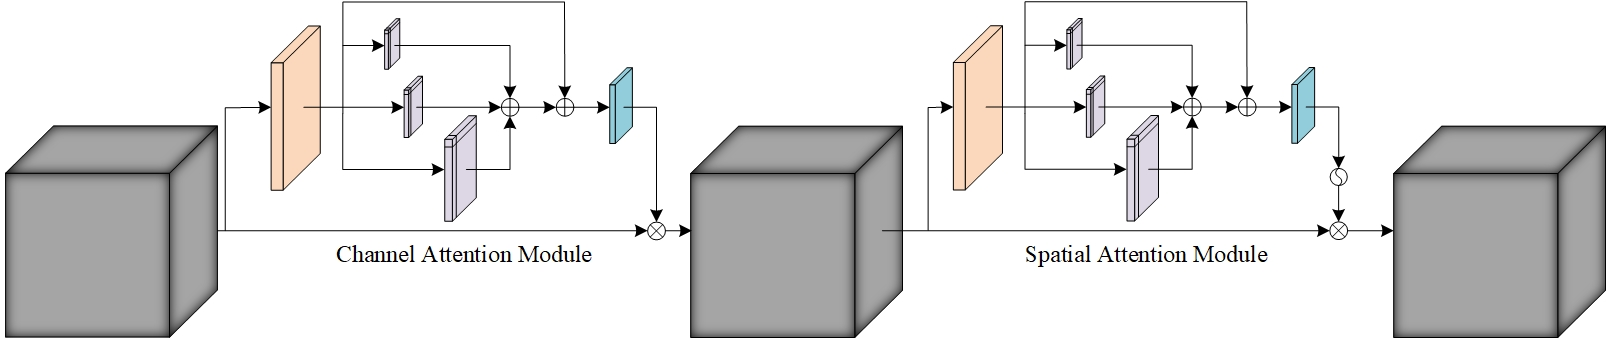
\includegraphics[width=0.8\linewidth]{picture/LLIE/Experiment/Attention/CPMS}
			%\captionsetup{font=scriptsize}
			\caption{CPMS}
			\label{fig: CPMS}
		\end{figure}
		
		
		\subsection*{对UNet网络的改进方法}
		
		我们尝试了不同的 Encoder 和 Decoder 组合,如 Fig. \ref{fig: Encoder and Decoder} 所示,对于 Encoder 部分,我们首先应用注意力机制(Attention),然后使用 $3 \times 3$ 的轴向深度可分离卷积 (Depthwise Separable Convolution),接着进行批标准化 (Batch Normalization) 和 $1 \times 1$ 卷积操作,最后通过最大池化 (MaxPooling) 进行特征压缩,最终使用 Sigmoid 激活函数。对于 Decoder 部分,我们首先将其与对应的 Encoder 的跳跃连接进行 Concat 操作,然后进行上采样 (Upsample) 操作,接着应用注意力机制 (Attention) ,再次使用 $3 \times 3$ 的轴向深度可分离卷积,再通过批标准化和 $1 \times 1$ 卷积操作,最终采用 PReLU 激活函数。
		
		\begin{figure}[htbp]
			\centering
			\begin{subfigure}{0.8\textwidth}
				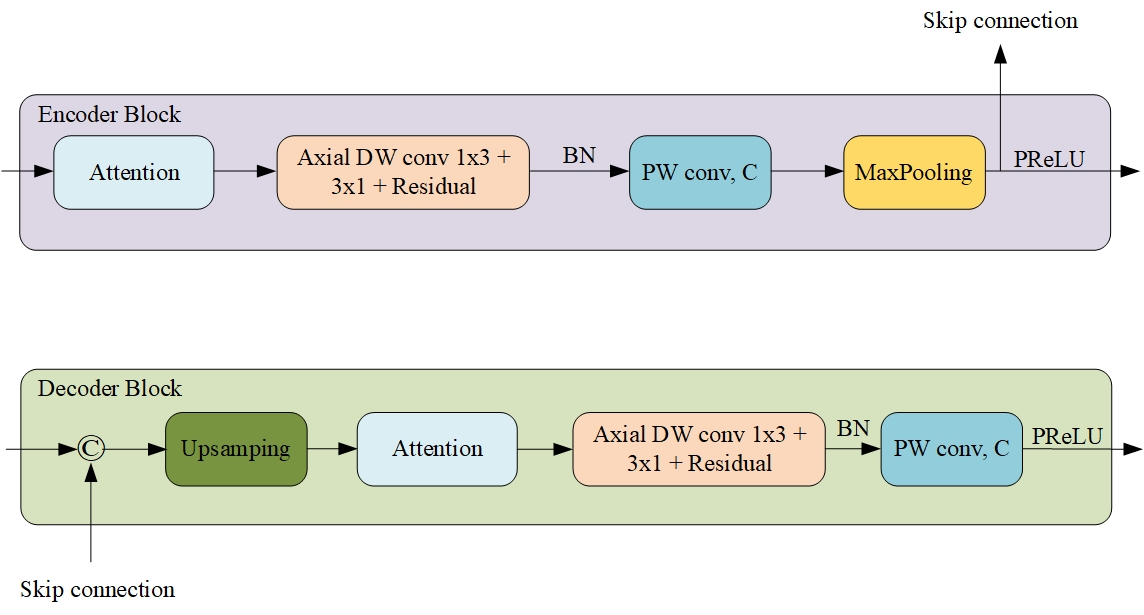
\includegraphics[width=\linewidth]{picture/LLIE/Experiment/Encoder and Decoder}
				\captionsetup{font=scriptsize}
				\caption{Encoder 和 Decoder 的搭配}
				\label{fig: Encoder and Decoder}
			\end{subfigure}
			\begin{subfigure}{0.8\textwidth}
				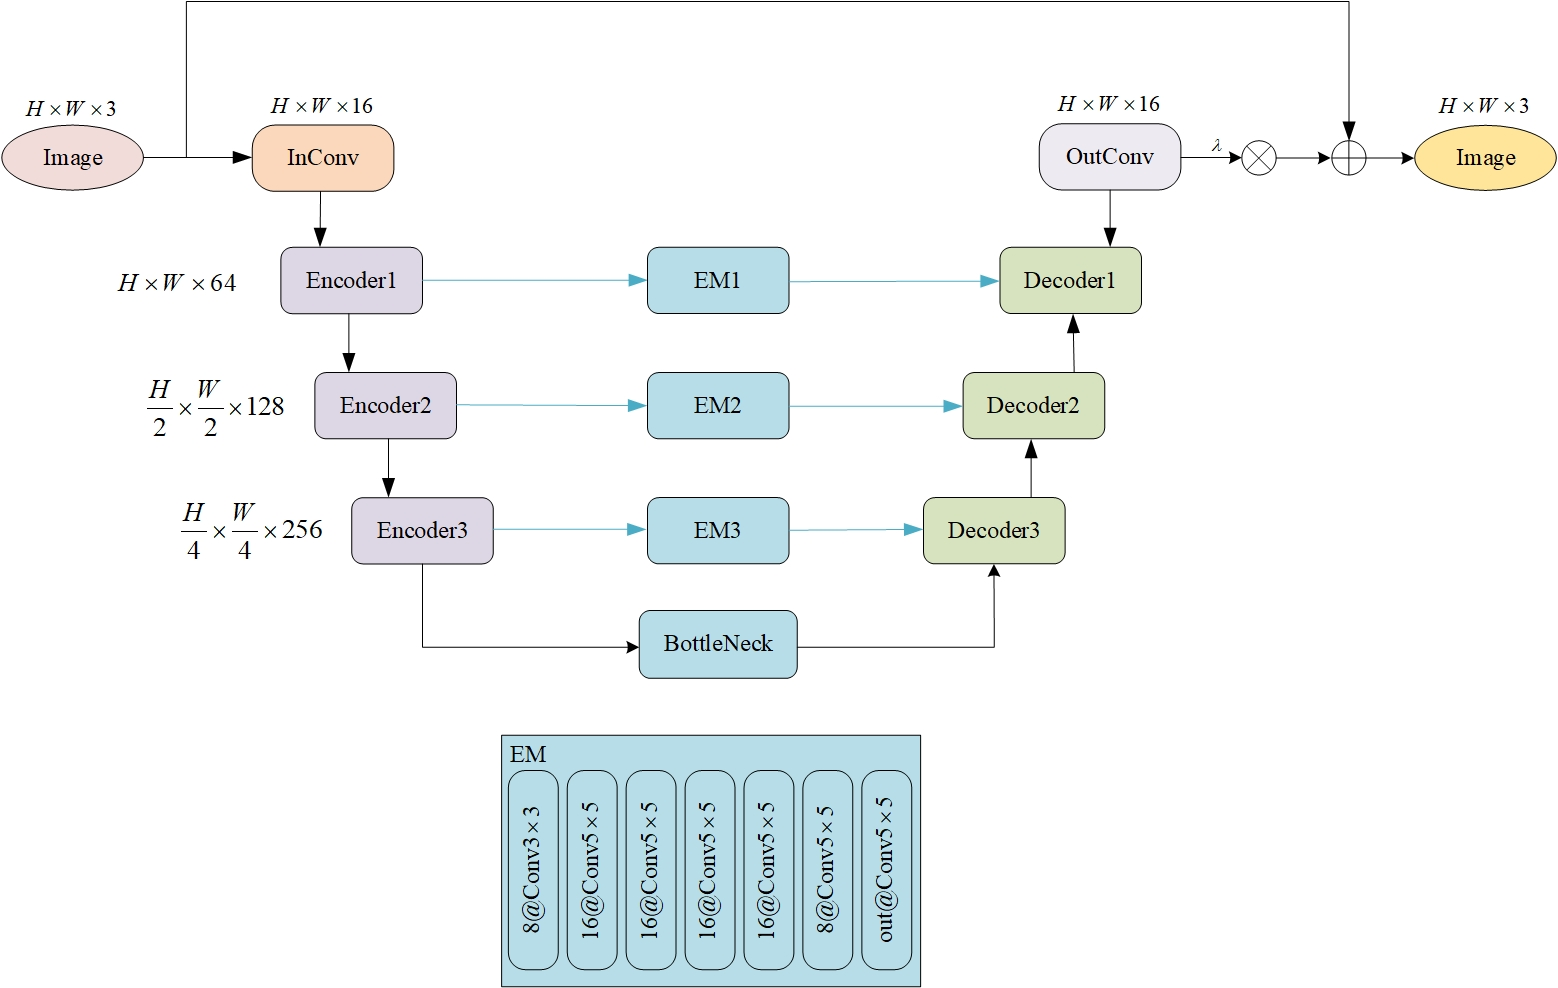
\includegraphics[width=\linewidth]{picture/LLIE/Experiment/Baseline}
				\captionsetup{font=scriptsize}
				\caption{我们提出的U-Net Baseline}
				\label{fig: Baseline}
			\end{subfigure}
		\end{figure}
		
		我们使用 MBLLEN\cite{lv2018mbllen} 中的 EM 模块,旨在加强每个层级中Encoder和Decoder之间的特征连接,从而增强模型的表现能力,如 Fig .\ref{fig: Baseline} 所示。

		
		我们将激活函数修改为 ReLU 和 PReLU, 其中可视化结果分别如 Fig. \ref{fig: Baseline_ReLU} 和 Fig. \ref{fig: Baseline_PReLU} 所示。
		
		\begin{figure}[htbp]
			\centering
			\begin{subfigure}{0.45\textwidth}
				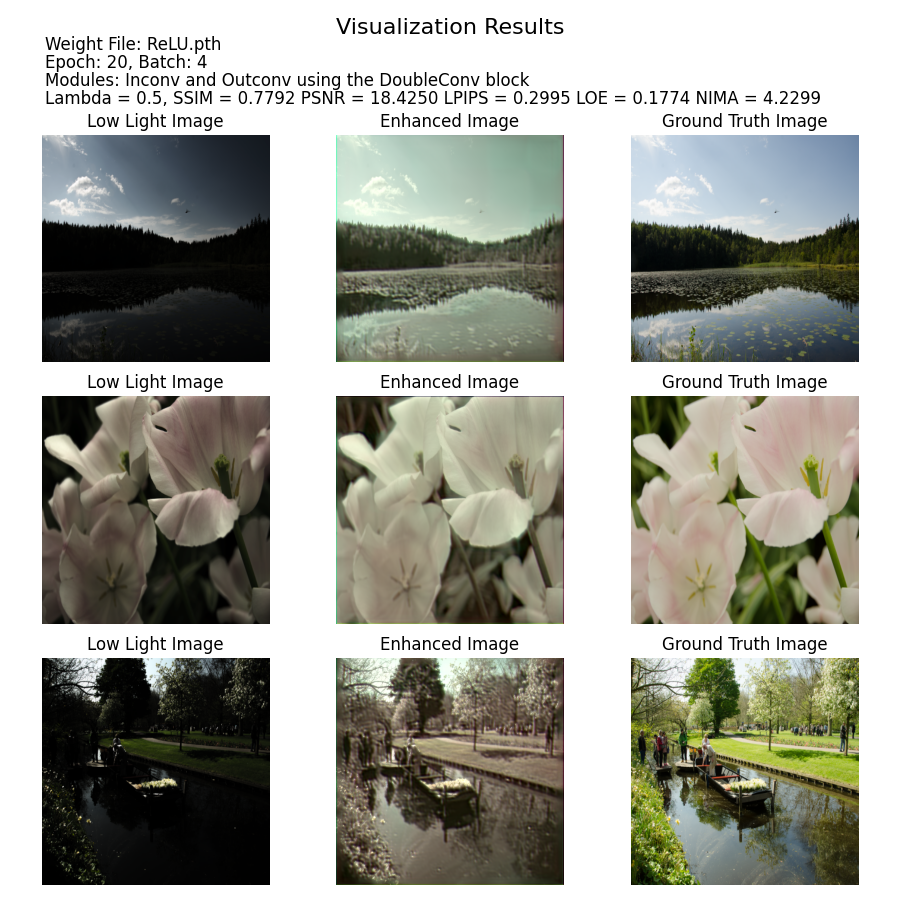
\includegraphics[width=\linewidth]{picture/LLIE/Experiment/myplot_UNet_ReLU}
				\captionsetup{font=scriptsize}
				\caption{ReLU}
				\label{fig: Baseline_ReLU}	
			\end{subfigure}
			\begin{subfigure}{0.45\textwidth}
				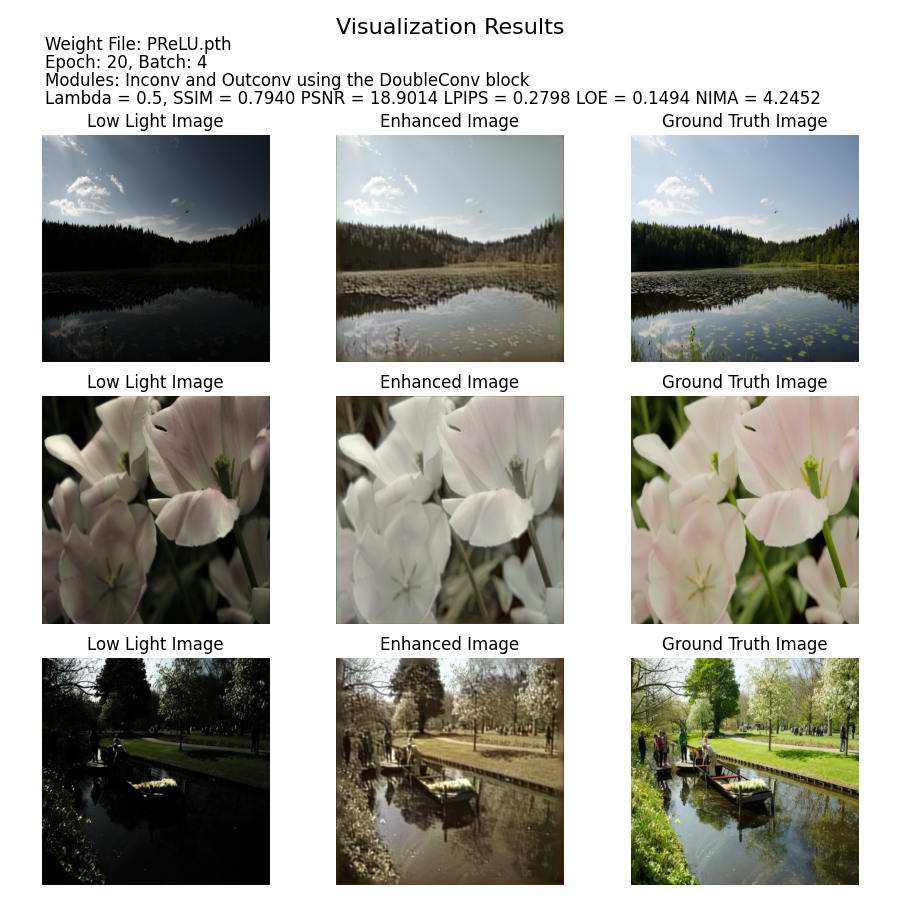
\includegraphics[width=\linewidth]{picture/LLIE/Experiment/myplot_UNet_PReLU}
				\captionsetup{font=scriptsize}
				\caption{PReLU}
				\label{fig: Baseline_PReLU}	
			\end{subfigure}
		\end{figure}
		
		\subsection{其他改进}
		
		\subsubsection{已知的点}
		
		\begin{itemize}
			\item{(1)}
			一般而言先使用残差块或改进的残差块再使用 Attention 块,主要是为了更好地进行跨通道和空间信息融合。
			
			\item{(2)}
			如果要做得更好,加入结构化先验最终的效果可能会更好。
			
			\item{(3)}
			目前只是针对残差网络上的改进可能意义不大,改进点更多聚焦于\textbf{特征提取能力},\textbf{模型轻量化},
			特征提取能力可以关注一下\textbf{图像超分或图像分割领域的算法,这些领域有针对于特征提取能力的一些相关研究}
		\end{itemize}
		
		\subsubsection{针对损失函数的改进}
		
		添加平滑度损失(Total Variation Loss)\cite{rudin1992nonlinear}, 受噪声污染的图像的总变分比无噪图像的总变分明显的大, 最小化TV理论上就可以最小化噪声。我们考虑到增强后的图像亮度是不连续的,可能会放大部分噪声,这会降低增强图像的质量,因此采用 TV Loss 约束增强图像。
		
		\begin{equation}
			\begin{aligned}
				\text{Loss}_{\text{TV}} \left( y \right) = \sum_{i=1}^{H} \sum_{j=1}^{W}\sqrt{\left(y_{i,j} - y_{i+1, j}\right)}			
			\end{aligned}
			\label{eq: TV loss}
		\end{equation}
		
		\FloatBarrier
		
		\subsubsection{针对亮度的改进}
		
		\paragraph{LBP}
		
		弱光图像和正常光照图像差距体现在像素值上的不同,即弱光数值低,正常光数值高,弱光图像增强任务可以看作是一个映射(Mapping),这个映射将弱光图像重建出正常光的图像,DLN\cite{DLN2020}中提出一种基于反投影理论 (Back-projection) 和注意力机制的但图像弱光图像增强方法。作者认为没有绝对的 NL (Normal lighting) 图像,NL 图像不过就是比 LL 图像像素值高一些,动态范围更大一些。受超分辨\cite{haris2018deep}的思想,希望利用反向投影从 LL 图像中重建出NL图像。 所以作者提出了 LBP (Lighting Back Projection) 模块(对特征图进行残差学习,增强明亮效果),和 FA(Feature Aggregation)模块 (重新校准特征图特征)。

		其中LBP模块如 Fig. \ref{fig: LBP},我们基于LBP模块设置了一个并行结构,如 Fig. \ref{fig: UNet and LBP} 所示。
		
		\begin{figure}[htbp]
			\centering
			\begin{subfigure}{0.8\textwidth}
				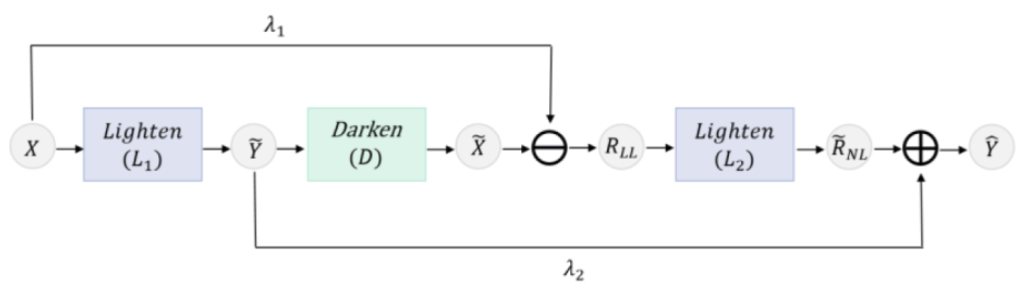
\includegraphics[width=\linewidth]{picture/LLIE/Experiment/LBP}
				\captionsetup{font=scriptsize}
				\caption{Lighting Back Projection}
				\label{fig: LBP}
			\end{subfigure}
			\begin{subfigure}{0.8\textwidth}
				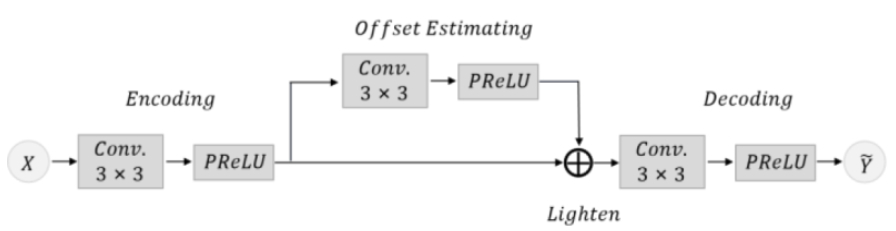
\includegraphics[width=\linewidth]{picture/LLIE/Experiment/Lighten operation}
				\captionsetup{font=scriptsize}
				\caption{Lighten operation}
				\label{fig: Lighten operation}	
			\end{subfigure}
			\begin{subfigure}{0.8\textwidth}
				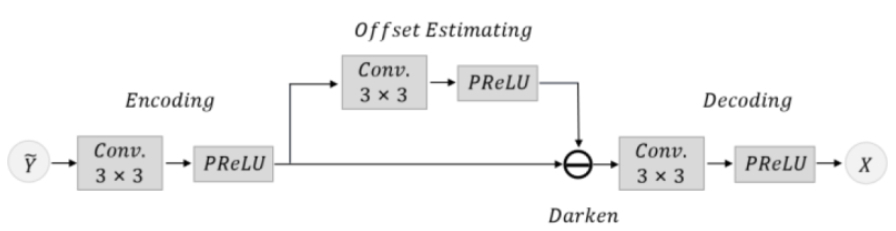
\includegraphics[width=\linewidth]{picture/LLIE/Experiment/Darken operation}
				\captionsetup{font=scriptsize}
				\caption{Darken operation}
				\label{fig: Darken operation}	
			\end{subfigure}
			\caption{图源自\cite{shen2022low}}
		\end{figure}
		
		\begin{figure}[htbp]
			\centering
			\begin{subfigure}{0.8\textwidth}
				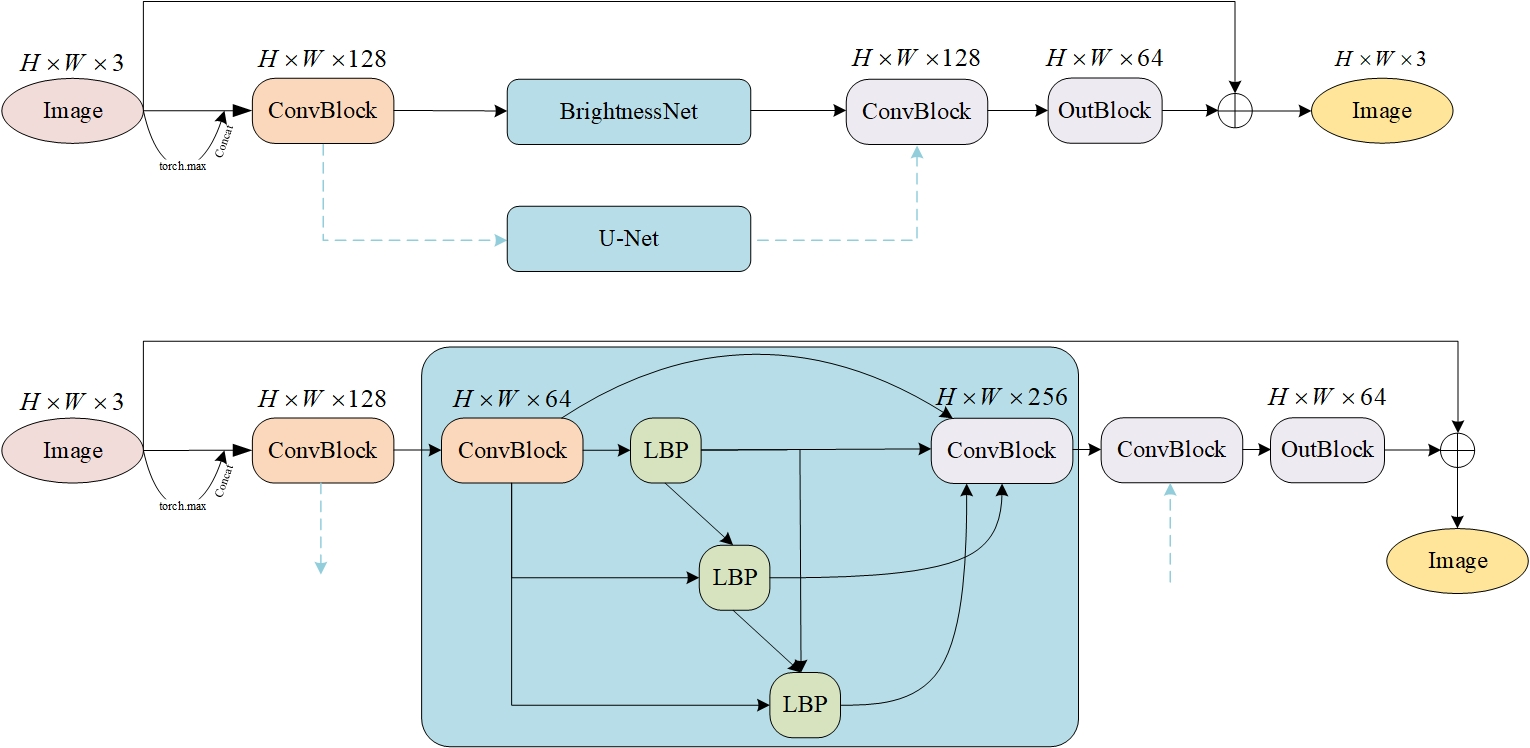
\includegraphics[width=\linewidth]{picture/LLIE/Experiment/UNet and LBP}
				\captionsetup{font=scriptsize}
				\caption{UNet and LBP}
				\label{fig: UNet and LBP}
			\end{subfigure}
			\begin{subfigure}{0.8\textwidth}
				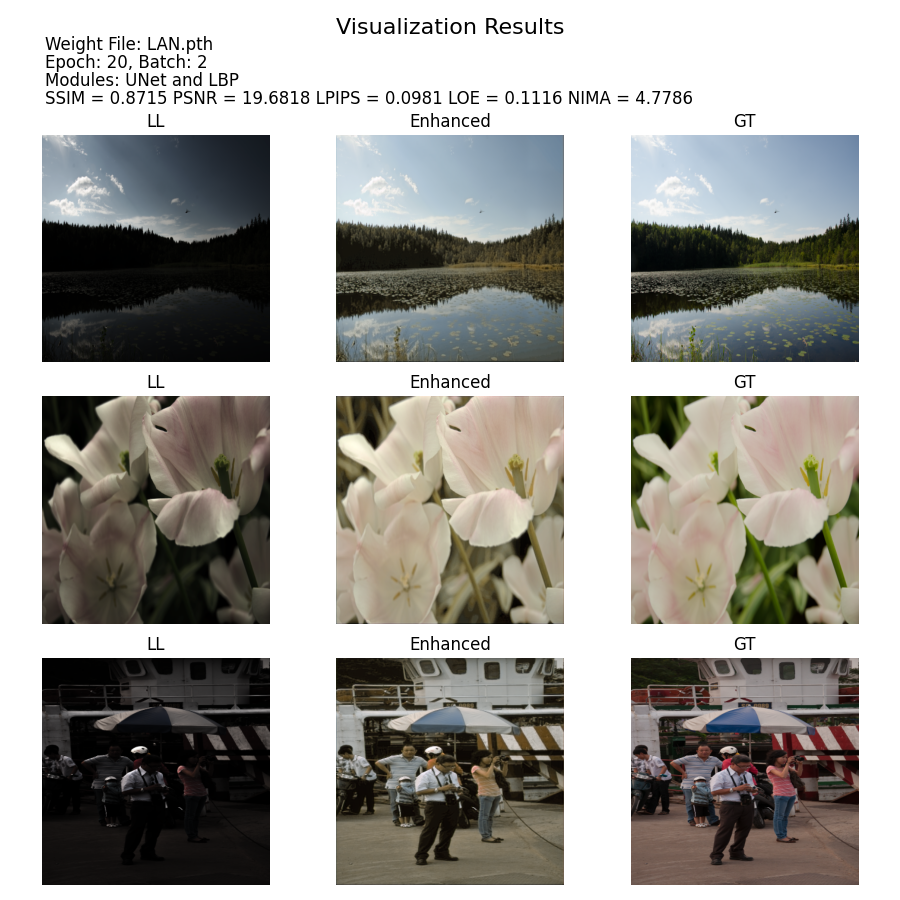
\includegraphics[width=\linewidth]{picture/LLIE/Experiment/myplot_LAN}
				\captionsetup{font=scriptsize}
				\caption{Lighten operation}
				\label{fig:myplot_LAN}
			\end{subfigure}
		\end{figure}
		
		增强结果如 Fig. \ref{fig:myplot_LAN}所示。
		
		\renewcommand{\refname}{References}
		
		
		%	\begin{thebibliography}{00}
			
			%		\bibitem{b1}\label{cite:b1}
			%		W. Wang, C. Wei, W. Yang and J. Liu, "GLADNet: Low-Light Enhancement Network with Global Awareness," 2018 13th IEEE International Conference on Automatic Face \& Gesture Recognition (FG 2018), Xi'an, China, 2018, pp. 751-755, DOI: 10.1109/FG.2018.00118.
			
			%		\bibitem{b2}\label{cite:b2}
			%		A.\ Mahajan, K.\ Somaraj and M. Sameer, "Adopting Artificial Intelligence Powered ConvNet To Detect Epileptic Seizures," 2020 IEEE-EMBS Conference on Biomedical Engineering and Sciences (IECBES), Langkawi Island, Malaysia, 2021, pp. 427-432, DOI: 10.1109/IECBES48179.2021.9398832.
			
			%		\bibitem{Cyr}
			%		N.\ Cyr, M.\ T$\hat{e}$tu, and M.\ Breton,
			% "All-optical microwave frequency standard: a proposal,"
			%		IEEE Trans.\ Instrum.\ Meas.\ \textbf{42}, 640 (1993).
			
			
			
			%	\end{thebibliography}
		
		\bibliographystyle{unsrt}
		\bibliography{reference}
		
		
	\end{document}
